%%%%%%%%%%%%%%%%%%%%%%%%%%%%%%%%%%%%%%%%%%%%%%%%%%%%%%%%%%%%%%%%%%%%%%%%%%%%%%%%%%%%%%%%%%%%%%%%%%%%%%%%%%%%%%%%%%%%%%%%%%%%%%%%%%%%%%%%%%%%%%%%%%%%%%%%%%%
% This is just an example/guide for you to refer to when submitting manuscripts to Frontiers, it is not mandatory to use Frontiers .cls files nor frontiers.tex  %
% This will only generate the Manuscript, the final article will be typeset by Frontiers after acceptance.   
%                                              %
%                                                                                                                                                         %
% When submitting your files, remember to upload this *tex file, the pdf generated with it, the *bib file (if bibliography is not within the *tex) and all the figures.
%%%%%%%%%%%%%%%%%%%%%%%%%%%%%%%%%%%%%%%%%%%%%%%%%%%%%%%%%%%%%%%%%%%%%%%%%%%%%%%%%%%%%%%%%%%%%%%%%%%%%%%%%%%%%%%%%%%%%%%%%%%%%%%%%%%%%%%%%%%%%%%%%%%%%%%%%%%

%%% Version 3.4 Generated 2018/06/15 %%%
%%% You will need to have the following packages installed: datetime, fmtcount, etoolbox, fcprefix, which are normally inlcuded in WinEdt. %%%
%%% In http://www.ctan.org/ you can find the packages and how to install them, if necessary. %%%
%%%  NB logo1.jpg is required in the path in order to correctly compile front page header %%%

\documentclass[utf8]{frontiersSCNS} % for Science, Engineering and Humanities and Social Sciences articles
%\documentclass[utf8]{frontiersHLTH} % for Health articles
%\documentclass[utf8]{frontiersFPHY} % for Physics and Applied Mathematics and Statistics articles

%\setcitestyle{square} % for Physics and Applied Mathematics and Statistics articles
\usepackage{url,hyperref,lineno,microtype,subcaption}
\usepackage[onehalfspacing]{setspace}
\epstopdfsetup{outdir=./}

\linenumbers


% Leave a blank line between paragraphs instead of using \\


\def\keyFont{\fontsize{8}{11}\helveticabold }
\def\firstAuthorLast{Mrad {et~al.}} %use et al only if is more than 1 author
\def\Authors{Assaad Mrad\,$^{1,*}$, Sanna Sevanto\,$^{2}$, Jean-Christophe Domec\,$^{1,3}$, Yanlan Liu\,$^{1}$, Mazen Nakad\,$^{1}$ and Gabriel Katul\,$^{1,4}$}
% Affiliations should be keyed to the author's name with superscript numbers and be listed as follows: Laboratory, Institute, Department, Organization, City, State abbreviation (USA, Canada, Australia), and Country (without detailed address information such as city zip codes or street names).
% If one of the authors has a change of address, list the new address below the correspondence details using a superscript symbol and use the same symbol to indicate the author in the author list.
\def\Address{$^{1}$Nicholas School of the Environment, Duke University, Durham, NC, USA \\
$^{2}$Earth and Environmental Sciences Division, Los Alamos National Laboratory, Los Alamos, New Mexico, USA \\
$^{3}$ UMR INRA-ISPA 1391, Bordeaux Sciences Agro, Gradignan 33195, France \\
$^{4}$Department of Civil and Environmental Engineering, Duke University, Durham, NC}
% The Corresponding Author should be marked with an asterisk
% Provide the exact contact address (this time including street name and city zip code) and email of the corresponding author
\def\corrAuthor{Assaad Mrad}

\def\corrEmail{mradassaad2@gmail.com}




\begin{document}
\onecolumn
\firstpage{1}

\title[Dynamic optimality principle for water use strategies]{A dynamic optimality principle for water use strategies explains isohydric to anisohydric plant responses to drought} 

\author[\firstAuthorLast ]{\Authors} %This field will be automatically populated
\address{} %This field will be automatically populated
\correspondance{} %This field will be automatically populated

\extraAuth{}% If there are more than 1 corresponding author, comment this line and uncomment the next one.
%\extraAuth{corresponding Author2 \\ Laboratory X2, Institute X2, Department X2, Organization X2, Street X2, City X2 , State XX2 (only USA, Canada and Australia), Zip Code2, X2 Country X2, email2@uni2.edu}


\maketitle


\begin{abstract}

%%% Leave the Abstract empty if your article does not require one, please see the Summary Table for full details.
\section{}
For full guidelines regarding your manuscript please refer to \href{http://www.frontiersin.org/about/AuthorGuidelines}{Author Guidelines}.

As a primary goal, the abstract should render the general significance and conceptual advance of the work clearly accessible to a broad readership. References should not be cited in the abstract. Leave the Abstract empty if your article does not require one, please see \href{http://www.frontiersin.org/about/AuthorGuidelines#SummaryTable}{Summary Table} for details according to article type. 


\tiny
 \keyFont{ \section{Keywords:} keyword, keyword, keyword, keyword, keyword, keyword, keyword, keyword} %All article types: you may provide up to 8 keywords; at least 5 are mandatory.
\end{abstract}

\section{Introduction}
Some two centuries after the seminal experiments of Francis Darwin \citep{darwin1898ix,scarth1927stomatal}, it is safe to state that the significance of stomatal kinetics in climate, atmospheric, hydrologic, agricultural, and ecosystem sciences is not in dispute \citep{hetherington2003role}.  The exchanges of water vapor and CO$_2$ between the atmosphere and plants are regulated by a dynamic stomatal aperture, which then directly impacts a plethora of processes such as CO$_2$ concentration in the atmosphere and any positive feedback on air temperature \citep{cox2000acceleration} as well as water cycling \citep{betts2007projected,katul2012evapotranspiration}, sensible heat flux and boundary layer dynamics regulating predisposition of rainfall \citep{siqueira2009soil, manoli2016soil}, pollutant uptake such as tropospheric ozone and concomitant plant damage \citep{rich1964ozone,musselman2006critical}, antecedent soil moisture content and flash-flooding \citep{javelle2010flash}, silviculture and forest management \citep{makela1986stand}, irrigation water requirements and profitable crop yield \citep{vico2015ecohydrology} to name a few.  What remains the subject of inquiry and continues to draw significant research attention is how to parsimoniously represent stomatal kinetics for the aforementioned plethora of applications. Numerous models for stomatal kinetics have emerged over the past century or so (for an overview see e.g. \citet{jarvis1976interpretation,interpretation_1976,collatz_physiological_1991,leuning_critical_1995,damour2010overview,way2011well} ). These studies, however, suggest that:  (i) stomatal kinetics cannot be considered in isolation as they are impacted by exogenous environmental variables \citep{jarvis1976interpretation,pearcy1990sunflecks,mott1991stomatal,medlyn_temperature_2002} such as photosynthetically active radiation (PAR), air temperature ($T_a$), vapor pressure deficit (VPD), atmospheric CO$_2$ ($c_a$), as well as other endogenous variables impacted by soil-plant processes such soil-plant hydraulics \citep{sperry_hydraulic_2000, brodribb_relations_2003}, osmoregulation and carbohydrate export from the leaf \citep{sevanto_how_2014,jensen2016sap,konrad2018xylem} to name a few; and  (ii) optimization principles based on maximum fitness offer a whole-systems framework to begin tackling the description of stomatal kinetics \citep{manzoni_optimizing_2011,manzoni_optimization_2013,huang2018transport}.  Because photosynthesis is the main source of carbon used by plants for growth and numerous vital functions  including plant defenses \citep{novick2012increased}, maximizing fitness is akin to maximizing photosynthesis over a preset time scale yet to be determined \citep{cowan1971relative,givnish1976sizes,cowan_stomatal_1977,dewar2010maximum}.  This approach is quite appealing because the mathematical framework to be employed (i.e., variational principles) has been developed and used in numerous branches of science.  \citep{witelski_variational_2015}.  The barriers to utilizing variational principles to describing stomatal kinetics is not in the formulation of the 'functional' to be maximized (i.e., photosynthesis) but in the constraints and costs to be imposed on such optimization \citep{dewar2018new}.  Naturally, those constraints and costs operate over time scales that may be difficult to determine a priori .  Early work on using variational principles focused on maximizing photosynthesis with costs (in carbon units) being set by transpirational losses from leaves at every instant \citep{cowan_stomatal_1977,cowan_stomatal_1978}.  Other versions of this maximization view stomata as 'autonomous' entities maximizing instantaneous carbon gain for a given finite amount of water loss \citep{katul_leaf_2009} so as to ensure stomata are open during stomatal movement.  A recent approach seeking instantaneous maximization of gains assumes that stomatal opening trends are controlled by plant hydraulics.  The approach is now labelled as a profit-maximization model for stomatal kinetics \citep{sperry_pragmatic_2016,sperry_predicting_2017}. In the profit-maximization scheme, the cost is formulated based on relative loss in plant hydraulic conductance whereas the gain is based on relative photosynthesis.  Other optimization variants have also been proposed based on maintaining constant inter-cellular to ambient atmospheric CO$_2$ concentration gradient \citep{prentice2014balancing}, or maximizing carbon transport out of the leaves through the phloem (Nikinmaa et al.).  In the constant CO$_2$ gradient approach, the objective is to minimize instantaneous cost (instead of maximize gains) of maintaining the transpirational stream required to support photosynthesis while maintaining photosynthetic proteins at levels required to support assimilation rates.  All these approaches have received experimental support under wide-ranging conditions despite differences in formulating costs  \citep{prentice2014balancing,sperry_predicting_2017}.
The past five decades have witnessed a renaissance in the development and use of optimization theories to describe stomatal kinetics by revising the nature of the costs associated with photosynthetic gains to include soil-plant hydraulics, soil water availability, energy limitations \citep{roth2018fossil} among others, and are all gaining prominence and partial experimental support.  What is clearly missing is a general framework that is able to recover the various optimization schemes already proposed and explicitly link these schemes with plant-water use strategies.  The work here aims to establish the blue-print of such a framework using plant hydraulics and droughts as case studies.  The focus on droughts here is purposeful because of the recent interest (and debates) about plant-water use strategies during droughts, and ways of defining and measuring isohydricity (refs).  Such analysis requires a re-formulation of the optimization problem to operate on a sub-daily time scale to explicitly accommodate variable environmental drivers and abiotic (e.g., drainage) as well as biotic (i.e., overlaping rooting zones of adjacent plants) competition for water. The theoretical framework to be employed is based on the calculus of variation and dynamic optimization principles because they allow for (i) directly accounting for plant-water use strategies (i.e. aggressive versus conservative water users), (ii) using multiple constraints (such as ...), and  (iii) extending the deterministic analysis used here to a stochastic framework (at least for rainfall) using conventional approaches  \citep{cowan1986economics,makela1996optimal,manzoni_optimization_2013,lu2016optim}.  is possible by assigning a 'carbon value' to the terminal soil moisture content around the rooting zone \citep{manzoni_optimization_2013},   Here we will focus on point (i) to demonstrate the power of this approach and leave points (ii) and (iii)  for future research.   
To guide the development of this framework, the work here answers the following question: To what degree does water use strategy (WUS) dictate stomatal control during dry-down? In a recent review of the theory of optimal stomatal control, \citet{buckley_optimal_2017} recognize the importance of delayed benefits such as keeping soil moisture at higher levels for future use, which is accommodated here via a terminal gain. The optimization scheme proposed here explores the consequences of WUS and choices made about soil-plant hydraulic strategy, and whether plant hydraulic traits alone are capable of mapping stomatal behavior anywhere on the iso-anisohydry spectrum. In particular, we study the model behavior in the water demand and supply limited cases, demonstrate the influence of competition on plant water use for trees of three different hydraulic vulnerability curves (VCs), and compare our approach with the combined plant hydraulic constraints and profit maximization approach.


\section{Materials and Methods}

\subsection{Theory: calculus of variations}

The principle adopted here is that plants maximize their carbon gain ($A$) over a known drydown period $T$ selected to be the mean inter-storm period. This principle assumes that plants freely control stomatal conductance $g_s$ per unit leaf area under constraints. Previous work constrained control of $g_s$ by enforcing the instantaneous water balance at the soil level \citep{manzoni_optimization_2013}. To mathematically express this principle and constraint, an augmented Lagrangian is defined $L$:
\begin{equation}
    \label{eqn:Lagrangian}
    L\Big(g_s, x, \frac{dx}{dt}, \lambda, t\Big) = A(g_s, t) - \lambda \Bigg[ \frac{dx}{dt} - f_e\Big(g_s, x, \frac{dx}{dt}, t\Big)\Bigg],
\end{equation}
where $\lambda$ is the Lagrange multiplier in mol mol$^{-1}$, $x$ is the relative soil moisture content or degree of saturation in the rooting zone, $t$ is time, and $f_e$ sums water inputs to the soil and subtracts outputs.

Because our approach states that $A$ is maximized over a period $T$ and not instantaneously, the objective function $J$ must be formed by time-integrating $L$ from $t=0$ signifying the beginning of a dry down to $t=T$ at the end of it:
\begin{equation}
    \label{eqn:Objective}
    J\Big(g_s, x, \frac{dx}{dt}, \lambda, t\Big) = \int_0^T L\Big(g_s, x, \frac{dx}{dt}, \lambda, t\Big).
\end{equation}
The goal then consists of finding the function $g_s(t)$ in terms of $t$ that maximizes $J$ over the period $T$. This goal is achieved by solving the so-called Euler-Lagrange equations using the calculus of variations. A required step however is expressing $A$ and $f_e$ in terms of the control variable $g_s$ and the state variable $x$, which are now discussed.

\subsection{Carbon gain}

The biochemical demand for atmospheric CO$_2$ for a C3 leaf is either limited by the Ribulose-1,5-bisphosphate carboxylase/oxygenase (Rubisco) enzyme activity under saturated incoming PAR or by Ribulose-1,5-biphosphate (RuBP) activity under limiting incoming PAR \citep{farquhar_biochemical_1980}. To avoid the use of non-differentiable functions, $A_{demand}$ is approximated using \citep{vico_perspective_2013}:
\begin{equation}
    \label{eqn:vico_model}
    A_{demand} = k_1 \frac{c_i - \Gamma^*}{c_i + k_2},
\end{equation}
where $c_i$ is the carbon dioxide concentration in the intercellular spaces of the leaf assumed to be equal to the concentration inside the chloroplast (infinite mesophyll conductance), $k_1$ and $k_2$ are parameters determined from limits imposed on $c_i$ as described elsewhere \citep{vico_perspective_2013}. Namely, $k_1 = \frac{J}{4}$ and $k_2 = \frac{J}{4} \frac{a_2}{V_{c,max}}$, and $\Gamma^*$ is the CO$_2$ compensation point defined by the $c_i$ where carbon dioxide assimilation rate ceases. The carbon dioxide concentration inside the chloroplast is used instead of the one inside the leaf because this model is calculating the carbon demand of the chlorophyll.

Equation \ref{eqn:vico_model} is of a Michaelis-Menten type where $k_1$ is interpreted as the maximum rate of carbon dioxide assimilation and $k_2$ prescribes the strength of the carboxylation compared to oxygenation through $a_2$. The $a_2 = K_c (1+O_a/K_o)$ where $K_c$ and $K_o$ are Michaelis-Menten constants for CO$_2$ and O$_2$ respectively and $O_a$ is the atmospheric concentration of oxygen.

The parameters of equation \ref{eqn:vico_model} ($V_{c,max}$, $\Gamma^*$, $K_c$, $K_o$) are temperature dependent while $J$ is both $T_a$ and PAR dependent \citep{medlyn_temperature_2002}. The formulations describing the dependence of $K_c$, $K_o$, and $\Gamma^*$ on $T_a$ are conventional and are described elsewhere for transgenic tobacco \citep{bernacchi_improved_2001}. $J_{max}$ and $V_{c,max}$ dependencies on $T_a$ are taken from prior studies for \textit{Pinus pinaster} \citep{medlyn_temperature_2002} while the optimal values $J_{opt}$ and $V_{c,opt}$ were altered to match those of \text{Pinus ponderosa} at 25 degrees Celsius, the dominant species in the ecosystem of interest (ref).

For simplicity, the approximations used for $A_{demand}$ in equation \ref{eqn:vico_model} neglect 1) the potential limitation by sucrose synthesis, 2) the contribution by dark respiration to $A_{demand}$, and 3) the temperature buffering effect of the leaf boundary layer such that leaf temperature is set to atmospheric temperature $T_a$.  The latter approximation avoids the need for specifying wind speed variations and turbulent intensity within the canopy.

When every CO$_2$ molecule captured from the atmosphere by the leaf is assimilated, $A_{demand} = A_{supply}$. The supply of carbon dioxide from the atmosphere into the intercellular space is represented by a Fickian diffusion  with a diffusivity that depends on stomatal kinetics:
\begin{equation}
    \label{eqn:supply}
    A_{supply} = g_s (c_a - c_i),
\end{equation}
where $c_a$ is, as before, the atmospheric concentration of CO$_2$ in mmol mol$^{-1}$.

To determine the carbon dioxide concentration inside the chloroplast, we adopt a relation developed elsewhere \citep{dewar2018new}:
\begin{equation}
    \label{eqn:dewar_mes}
    c_c - \Gamma^* = \varphi(c_i - \Gamma^*)
\end{equation}
where $\varphi = 1 - \frac{\psi_l}{\psi_c}$ is used as a reduction factor and $\psi_c$ is the critical leaf water potential whose numerical value is defined below and $\psi_l$ is the actual leaf water potential. 
Combining equations \ref{eqn:vico_model}, \ref{eqn:supply} and \ref{eqn:dewar_mes}, a formulation for $A$ in terms of $g_s$ that is explicitly independent from $c_c$ is obtained and given as:
\begin{equation}
    \label{eqn:A_noci}
    A = k_1\frac{[(\Gamma^* - c_a)\varphi + k_2 + \Gamma^*]g_s + k_1\varphi - \sigma}{[(\Gamma^* - c_a)\varphi - k_2 - \Gamma^*]g_s + k_1\varphi - \sigma},
\end{equation}
where $\sigma = \sqrt{[(c_a - \Gamma^*)\varphi + k_2 + \Gamma^*]^2g_s^2 + 2{\varphi}{k_1}[(\Gamma^* - c_a)\varphi + k_2 + \Gamma^*]g_s + k_1^2\varphi^2}$.  Because $\sigma$ is positive, the $A$-$g_s$ relation is a concave function, a necessary condition for optimal behavior as discussed elsewhere \citep{katul_stomatal_2009}.

To sum up, when the temporal variations in $T_a$ and PAR are specified along with $c_a$ and $O_a$, then $g_s$ is the only independent variable in equation \ref{eqn:A_noci}.

\subsection{Soil water balance}

% The ensure the continuity of the water stream throughout the tree, we model three vertically connected layers: the soil, the trunk and branches, and the leaves. Each of these layers are characterized by a hydraulic resistance that is non-linearly related to water potential. Prescribing hydraulic resistances to these different layers allows computation of quantities regarded as indicative of isohydric to anisohydric behaviour. Such quantities include leaf water potential ($\psi_l$) and stomatal conductance ($g_s$).

During a dry-down, precipitation is absent and the hydrologic balance can be expressed as \citep{rodriguez-iturbe_ecohydrology_2007}:
\begin{equation}
    \label{eqn:soil_water}
    \frac{dx(t)}{dt} = f_e\Big(g_s, x, \frac{dx}{dt}, t\Big) = \frac{\nu}{ n Z_r}[- E(g_s, t) - U(x, t)],
\end{equation}
where $U$ lumps all the uncontrolled losses (independent of the plant) in mmol m$^{-2}$ s$^{-1}$, and E is the transpiration rate from the plant in mmol m$^{-2}$ s$^{-1}$ (throughout, water fluxes are expressed per unit leaf area),  $n$ is the soil porosity in m$^3$ m$^{-3}$ and $Z_r$ is the effective plant rooting depth in $m$. This balance must be satisfied at every instant $(t \in [0,T])$.  To ensure dimensional equivalence, the right hand side is multiplied by $\nu = \text{LAI} \, M_w/ \rho_w$, LAI is the leaf area index in m$^3$ m$^{-3}$, $M_w = 18 \times 10^{-6}$ kg mmol$^{-1}$ is the molar weight of water, and $\rho_w = 1000$ kg m$^{-3}$ is its density. The $U$ may account for both soil leakage away from the rooting zone and competition from other plant roots.  

Soil leakage is modeled as gravitational drainage such that water losses from leakage per unit soil area and per unit depth is determined by the soil hydraulic conductivity $g_x$ \citep{campbell_introduction_2012}:
\begin{equation}
    \label{eqn:soil_cond}
    g_x = g_{x,sat}x^{2b+3},
\end{equation}
where $g_{x,sat}$ is the soil conductivity at saturation and $b$ is a parameter determined from the soil water retention curve. Both parameters depend on pore structure that is linked to soil type using standard equations \citep{clapp_empirical_1978}. The soil water potential ($\psi_x$) can also be derived from the aforementioned soil water retention curve using:
\begin{equation}
    \label{eqn:Clapp_pot}
    \psi_x = \psi_{x,sat}x^{-b},
\end{equation}
where $\psi_{x,sat}$ is the soil water potential near field capacity.

The soil to root conductance $g_{sr}$ is assumed to be the conductivity of the soil $g_x$ divided by the distance between soil and root $l_{sr}$. $l_{sr} = \sqrt{d_r Z_r \text{RAI}}$ where $d_r$ is the fine root diameter in m and RAI is the root area index \citep{manzoni_optimization_2013}. If $g_x$ is given in kg s m$^{-3}$, then
\begin{equation}
    \label{eqn:soil_root}
    g_{sr} = \frac{10^9}{M_w \, \rho_w \, l_{sr} \, \text{LAI}} g_x, 
\end{equation}
where $g_{sr}$ now has units of mmol m$^{-2}$ MPa$^{-1}$ s$^{-1}$ and is expressed per unit leaf area again. Because the soil to root distance is taken into account in $g_{sr}$, one only needs to multiply $g_{sr}$ by the water potential difference between root and soil to obtain the flux of water from the soil into the roots.
\subsection{Leaf-level water balance}

As a point of departure from previous analyses based on carbon gain maximization principles, it is recognized here that plant transpiration must be limited by soil-plant hydraulics when atmospheric water demand exceeds the supply of water provided by the soil. This limitation imposes an upper bound on $g_s$. 

The loss of conductivity of the whole plant system with respect to water potential is described by an effective vulnerability curve (VC). For simplicity, we approximate the VC of the entire hydraulic pathway (roots, trunk, and branches) with a generic Weibull exceedance function \citep{sperry_predicting_2017} given by:
\begin{equation}
    \label{eqn:root_leaf}
    g_{rl} = g_{rl,max}exp\Big[-\Big(\frac{\psi}{\psi_{63}}\Big)^s\Big],
\end{equation}
where $g_{rl}$ is the root to leaf hydraulic conductance in mmol m$^{-2}$ MPa$^{-1}$ s$^{-1}$ expressed per unit leaf area, and $g_{rl,max}$ is its maximum value at saturation. The $\psi_{63}$ is the water potential at which the plant loses about 63\% of its conductance, as common in Weibull VCs. Finally, $s$ dictates the shape and curvature of the Weibull function. 
% To find $\psi_{p}$, we invoke the hydrostatic approximation between leaves and roots which leads to $\psi_{p}=\frac{\psi{r}+\psi_l}{2}$ where $\psi_r$ is the root water potential.
The $E$ at the soil, plant, and leaf levels are now expressed ass:
\begin{equation}
    \label{eqn: mass_cons}
        \begin{split}
        E & = E_{demand} = 1.6\: g_s\, \text{VPD} \\
        & = E_{sr} = g_{sr}(\psi_x)(\psi_x - \psi_r)\\
        & = E_{rl} = \int_{\psi_l}^{\psi_r} g_{rl}(\psi) d\psi. \\
        \end{split}
\end{equation}
Here, $E_{demand}$ is the atmospheric demand of water, $E_{sr}$ is the soil to root water supply, $E_{rl}$ is the root to leaf supply. All expressions of $E$ are given in units of mmol m$^{-2}$ s$^{-1}$ expressed per unit leaf area. The $E_{rl}$ expression is analogous to porous media methods where it is recognized that water potential is not distributed hydrostatically along the medium.

It is noted that as $g_s$ varies with time, $\psi_l$ also varies in time to match supply and demand. The hydraulic constraint from the plant water supply system is apparent when one realizes that while $E_{demand}$ is always increasing with $g_s$ for constant VPD, water supply through $E_{sr}$ and $E_{rl}$ have maxima that cannot be exceeded due to decreases in hydraulic conductance functions $g_{sr}$ and $g_{rl}$ with increasing $\psi_x$, $\psi_r$, and $\psi_l$ (equations \ref{eqn:soil_root}, \ref{eqn:root_leaf}, and \ref{eqn: mass_cons}). The presence of a maximum possible water supply imposes an additional constraint on the stomatal conductance $g_s$.  In fact, the essence of the previous profit maximization schemes is that this constraint dictates the transpiration and assumes plants always take full advantage of their transpirational capacity.

Our approach can impose this constraint with the help of another Lagrange multiplier. However, to maintain traditional definitions of marginal water use efficiency \citep{cowan_stomatal_1977}, the additional constraint is imposed differently. Specifically, if maximizing $J$ (equation \ref{eqn:Objective}) leads to a $g_s$ that exceeds the maximum achievable $E$ at current $x$, then this $g_s$ is replaced by finding the maximum transpiration rate \Big(at $\frac{\partial E}{\partial \psi_l} = 0$\Big). Hence, here the assumption that plants take full advantage of their maximum transpiration capacity only applies to those intervals when $g_s$ exceeds the maximum achievable $E$ at current $x$.

\subsection{Maximizing the objective}

From the definition of $J$ (equation \ref{eqn:objective}), there are 5 independent variables: $g_s$, $x$, $dx / dt$, $\lambda$, and $t$. To maximize $J$, the calculus of variations \citep{witelski_variational_2015} is used to derive what are known as the Euler-Lagrange equations (see equation 3.55 in the mentioned reference). For this problem, these are a set of three equations to be simultaneously solved with two boundary conditions set on $x$ at the beginning ($x(0)$ at $t=0$) and end of the drydown period ($x(T)$ at $t=T$). Solving this equations will yield the trends of the 5 independent variables with time so as to maximize $J$.

The use of this method leads to the so-called control equation,
\begin{equation}
    \label{eqn:control}
    \frac{\partial L}{\partial g_s} = \frac{\partial A}{\partial g_s} + \lambda \frac{\partial f_e}{\partial g_s} = 0,
\end{equation}
which gives a monotonic inverse relation between $\lambda$ and $g_s$ (see Results). One views equation \ref{eqn:control} as a control equation because we are taking the derivative of $L$ with respect to $g_s$ and $g_s$ "controls" the rate of soil water loss through transpiration. 

The so-called co-state equation is $\frac{\partial L}{\partial x} - \frac{d}{dt} \Big(\frac{\partial L}{\partial x'} \Big) = 0$, where $x'= \frac{dx}{dt}$ is used for notational consistency with \citet{witelski_variational_2015}. The co-state equation yields the time variation of $\lambda$,
\begin{equation}
    \label{eqn:co_state}
    \frac{d \lambda}{dt} = - \frac{\partial A}{\partial x} + \lambda \frac{\partial f_e}{\partial x} = \lambda \frac{\nu}{n\, Z_r} \frac{\partial U}{\partial x}.
\end{equation}
Finally, the sate equation, $\frac{\partial L}{\partial \lambda} = 0$ provides the soil water balance (equation \ref{eqn:soil_water}). In this context, the state $\lambda$ is known as the instantaneous marginal water use efficiency in ecological terms. It is to be noted that if $x$ does not vary appreciably in time or varies on time scales much longer than $g_s$, then $\partial U/{\partial x} = 0$ and $d\lambda/dt=0$ or, simply put, $\lambda = constant$.  This simplification for $x$ recovers the original arguments put forth by Cowan, Givnish, Farquhar and many others \citep{cowan_stomatal_1977,hari1986optimal,konrad2008modelling,katul_stomatal_2009,medlyn2011reconciling}.  The evaluation of this constant can no longer be provided by boundary conditions applied to the soil moisture balance and this constant must now be evaluated separately or determined empirically \citep{manzoni_optimization_2013}.  

Another major departure from prior optimization studies is the inclusion of the boundary conditions: equations \ref{eqn:control}, \ref{eqn:co_state}, and \ref{eqn:soil_water} are to be solved with preset initial and terminal soil moisture as noted before:
\begin{equation}
    \label{eqn: BC_no_WUS}
    \begin{split}
        BC_1 &:x(0)\\
        BC_2 &:x(T)\\
    \end{split}
\end{equation}
In reality, it is impossible to set a terminal soil moisture a priori. However, this can be amended by introducing a pre-set water use strategy (WUS), which is another novelty of the method proposed here.

\subsection{Water use strategy (WUS)}

To avoid setting $x(T)$ a priori, a terminal gain term is added to $J$ \citep{manzoni_optimization_2013}. The revised objective function $J$ is now :
\begin{equation}
    \label{eqn:objective}
    J_{WUS} = \int_0^{T_f} L\Big(g_s, x, \frac{dx}{dt},\lambda,t \Big) dt + J_{T},
\end{equation}
where $J_{T}$ may be interpreted as the carbon value of the terminal soil water moisture $x(T)$ prescribed as:
\begin{equation}
    \label{eqn:terminal_gain}
    J_{T} = \Lambda x(T),
\end{equation}
where $\Lambda$ in mol mol$^{-1}$ sets the carbon value of $x(T)$. Deriving the Euler-Lagrange equations once more to maximize $J_{WUS}$ gives the same differential equations (equations \ref{eqn:soil_water}, \ref{eqn:control}, \ref{eqn:co_state}). The main difference is that the boundary condition at $t=T$ is now set on $\lambda$ instead of $x(T)$: 
\begin{equation}
\label{eqn: BC_WUS}
    \begin{split}
        BC_1 &:x(0)\\
        BC_2 &:\lambda(T) = \Lambda.\\
    \end{split}
\end{equation}

A large $\Lambda$ allows mathematically setting a conservative WUS.  Conversely, setting $\Lambda$ to a small value allows mathematically setting an aggressive WUS for the plant. This approach departs from the assumption that carbon gain trends are instantaneously optimal for all plants because residual soil moisture at the end of dry-down now has a carbon value set by $\Lambda$. The presence of $J_{T}$ in equation \ref{eqn:objective} represents an opportunity cost, measured in carbon gain units, of depleting the soil of water and increasing cavitation on the short term.

The new optimization theory here accommodates short-term variability in environmental drivers, allows a prescribed vulnerability curve for the same long-term strategy ($\Lambda$), and vice versa. This description can discern the simultaneous effects of long-term WUS and concomitant VCs as well as as sub-daily fluctuations in environmental drivers on optimal trajectories of stomatal behavior $g_s(t)$.  Also, because the definition of $\lambda$ here purposely maintains its conventional form, diurnal evolution of $\lambda$ can be predicted in a manner consistent with the long-term WUS imposed by the conditions $\lambda(T)=\Lambda$ and $x(0)$ being specified.  A number of experiments reported variability in measured $\lambda=(\partial A/\partial g_s)/(\partial E_{demand}/\partial g_s)$ during the course of a day and argued that such variability is evidence against optimal stomatal functioning \citep{fites1988co2}.  The dynamic optimality approach proposed here makes clear that optimal stomatal functioning and short-term (sub-hourly) variability in $\lambda$ are expected.

\subsection{Environmental data} 
The model requires diurnal variations of the environmental variables including VPD, incident leaf shortwave radiation ($R_l$) or PAR, and $T_a$. The measurements provided by FLUXNET2015 dataset (DOI: 10.18140/FLX/1440068) at Blodgett forest are used as case study as this forest is known to experience episodic droughts. A drydown period starting on May 29, 2005 was chosen and the environmental variations over $100$ days are averaged into one representative day featuring the ensemble dirunal variations. These diurnal conditions are then repeated and tiled to all days defining the period $T$. This repeating pattern of diurnal environmental conditions allows isolating plant hydraulics and WUS form day-to-day variations in environmental drivers.

The work here neglects high-frequency changes in environmental variables (e.g. those commensurate to turbulent time scales that may range from fractions of seconds to minutes) as well as those occurring over monthly and longer times scales such as changes in leaf nitrogen, RAI, LAI, or VCs. As a compromise $T$ is selected to be on the order of 10 days or so and environmental variables are averaged over 0.5 h time scales.

The most abundant species at this site is \textit{pinus Ponderosa}. We therefore used temperature response curves for $V_{c,max}$ and $J_{max}$ of \textit{Pinus pinaster} from \citep{medlyn_temperature_2002} and shifted the whole curve such that their values at 25 degrees Celcius correspond the ones reported elsewhere at Blodgett forest for \textit{Pinus ponderosa} \citep{panek2004ozone}.

\section{Results}

\subsection{Demand driven transpiration}

Equation \ref{eqn:control} provides a functional dependence between $g_s$, $\lambda$, and environmental variables \citep{katul_stomatal_2009}:
\begin{equation}
    \label{eqn:gs_vs_env_lambda}
    \begin{split}
        g_s = & - \frac{k_1 (k_2-c_a+2 \Gamma^*)}{(k_2+c_a)^2} \\
        & +\frac{\sqrt{a\, \text{VPD}\, \lambda\, k_1^2 (c_a-\Gamma^*)(k_2+\Gamma^*)(k_2+c_a-2 a\, \text{VPD}\, \lambda)^2(k_2+c_a-a\, \text{VPD}\, \lambda)}}{a\, \text{VPD}\, \lambda (B - \Gamma^* +c_a)^2(B - \Gamma^* +c_a-a\, \text{VPD}\, \lambda)} ,
    \end{split}
\end{equation}
where $g_s$ is defined per leaf area as before. Sensitivity analysis reveals that the most influential atmospheric variable is VPD. The $g_s$ vs $\lambda$ phase space is featured for multiple VPD values (figure \ref{fig:gs_E_lam}a).  The $T_a$ and PAR and therefore $k_1$, $k_2$, and $\Gamma^*$ are set to their noon values (figure \ref{fig:environment}).

While this phase space is static in terms of $T_a$ and PAR, the dynamics of $g_s$ in response to $\lambda$ and VPD shown stay the same. In the case where water supply is not limited by the rhizosphere or the plant water pathway (equations \ref{eqn:soil_root}, \ref{eqn:root_leaf}), $g_s$ decreases as the air dries (and VPD increases) and vice versa for constant $\lambda$ (figure \ref{fig:gs_E_lam}a). This vertical movement of $g_s-\lambda$ state along the phase space closely resembles what happens on a sub-daily timescale when $\lambda$ does not vary appreciably. This is one driver of the midday stomatal closure when VPD is higher at midday compared to the morning and evening.

Another reason for a constant $\lambda$ could be the absence of uncontrolled losses $U$ (equation \ref{eqn:co_state}). If competitive water sinks such as other plants or leakage do exist, and the day to day change in VPD is minimal, then $g_s$ also decreases due to an increase in $\lambda$ albeit over a larger time scale of around 24 hours. This large time scale is mainly to allow $\lambda$ to change significantly. Realistically, droughts are accompanied with progressively drier air such that the combination of an increase of day to day VPD and an increase in $\lambda$ lead to a steeper decline in $g_s$ compared to the isolated action of these two effects.

Figure \ref{fig:gs_E_lam} elucidates how transpiration demand through VPD can drive the midday stomatal closure at the sub-daily and day to day time scales. For example, for demand driven transpiration and a constant $\lambda=12$ mmol mol$^{-1}$, a VPD$=8$ mmol mol$^{-1}$ corresponds to a $g_s\approx 40$ mol m$^{-2}$ s$^{-1}$. If at midday the VPD is doubled to 16 mmol mol$^{-1}$, $g_s$ becomes 0 indicating full stomatal closure and a 100\% decrease. If however, $\lambda=5$ mmol mol$^{-1}$, then for the same VPD change $g_s$ moves from $\approx 81$ mol m$^{-2}$ s$^{-1}$ to $\approx 43$ mol m$^{-2}$ s$^{-1}$, a noticeable but less aggressive decrease in $g_s$ of $\approx$ 47\%. However, larger PAR and $T_a$ could buffer that decrease in $g_s$ around noon by accelerating the chemical reactions visible through increases in $k_1$ and $k_2$ (equation \ref{eqn:A_noci}).

%  Another cause for an increase in $\lambda$ following this solid arrow is an increasingly supply-limited transpiration stream through the rhizosphere and the plant (an increase in PLC; equation \ref{eqn:supply}). This is seen by noticing that the solid arrow has a strong component normal to the lines of constant transpiration represented by red dashed lines in figure \ref{fig:gs_lam}. If however the changes in VPD are faster that changes in PLC then $g_s$ and $\lambda$ dynamics follow the short-dashed two-sided arrow that follows transpiration isolines. 

\subsection{Supply limited transpiration}

Supply limited transpiration occurs when the plant water pathway is inhibited enough by cavitation or when the soil is dry enough to set upper limits on $E$. This upper limit is labeled $E_{max}$ and defines transpiration rate that maximizes $g_s$, $\psi_r$, and $\psi_l$ at different $\psi_x$ (figure \ref{fig:gmax_Emax_psix}b,c). Figure \ref{fig:gmax_Emax_psix}a shows the partitioning of the total soil-root-leaf conductance into its soil-root and root-leaf components. Three VCs are compared in figure \ref{fig:gmax_Emax_psix} and they represent a resistant plant when $\psi_{63} = -3$ MPa, $s=4$, and $g_{rl,max} = 2$ mmol m$^{-2}$ MPa$^{-1}$ s$^{-1}$, a vulnerable plant when $\psi_{63} = -1.5$ MPa, $s=4$, and $g_{rl,max} = 2$ mmol m$^{-2}$ MPa$^{-1}$ s$^{-1}$, and an exponential plant when $\psi_{63} = -1$ MPa, $s=1$, and $g_{rl,max} = 8$ mmol m$^{-2}$ MPa$^{-1}$ s$^{-1}$. These three plants will be the same used in future comparisons throughout.

Because the $g_{sr}$ and $g_{rl}$ are in series, the total conductance from soil to leaf is limited by the lowest of the two. Therefore, the crossover point between $g_{sr}$ and $g_{rl}$ is a dynamically interesting point. Soil water conductance $g_x$ dependents on $\psi_x$ (equation \ref{eqn:soil_cond}) with the exponent $2b+3$ having a value of 9.1 for sandy loam \citep{campbell_introduction_2012}. This makes water movement from the soil to the roots a limiting factor at low soil moisture values. The crossover point occurs later for the exponential VC (at $\approx$ -0.5 MPa) compared to the other two plants (at $\approx$ -0.3 MPa) during a drydown. The location of this crossover point along the $\psi_x$ axis is also dependent on soil type and would occur at lower $\psi_x$ for more porous soil because of the stronger ensuing dependence of $g_x$ on $\psi_x$.

At drier soil, $g_{sr}$ becomes more limiting than $g_{rl}$ and forms a bottleneck to water supply to the leaves. Both the resistant and vulnerable plants experience a reduction in the $\psi_r - \psi_l$ difference as $\psi_x$ decreases to more negative values because maintaining a large difference would lead to only a negligible increase in water conductance of the whole hydraulic pathway (figure \ref{fig:gmax_Emax_psix}b). In contrast, this trend is absent for the plant with an exponential VC because the co-limiting state between $g_{sr}$ and $g_{rl}$ (figure \ref{fig:gmax_Emax_psix}a) allows $g_{rl}$ to influence total conductance as compared to the case of the resistant and vulnerable plants (figure \ref{fig:gmax_Emax_psix}b). Signs that plant hydraulics drive iso- and anisohydric behavior are becoming apparent already at this stage. When transpiration is supply limited, $\psi_l$ decreases with $\psi_x$ for an exponential VC such as in anisohydric plants (ref) compared to the more isohydric behavior of the resistant and vulnerable plants.

Figure \ref{fig:gmax_Emax_psix}c shows the transpiration rate of the soil-root-leaf pathway for the three plants. This figure accounts for $g_{sr}$ and $g_{rl}$ being driven by $\psi_x$, $\psi_r$, and $\psi_l$. Even though figure \ref{fig:gmax_Emax_psix}a shows that the exponential VC has the lowest overall minimizing conductance, it has the highest maximum transpiration rate of all three plants due to the fact that it can sustain $\psi_l$ as low as -9 MPa without experiencing a bottleneck for leaf water supply. So the greater difference between the aforementioned water potentials is what makes this exponential VC less limiting to transpiration.

If transpiration is truly supply limited, then $E_{max}$ determines the value of $\lambda$ in contrast to demand driven $E$. The blue dashed line in figure \ref{fig:gs_E_lam}b illustrates the case for the resistant plant when $E_{max}=0.2$ mmol m$^{-2}$ s$^{-1}$ at $\psi_x=-0.64$ MPa. This value of $E_{max}$ along with a VPD of 16 mmol mol$^{-1}$ leads to a $\lambda$ just under 10 mmol mol$^{-1}$. From figure \ref{fig:gs_E_lam}a, this value of $\lambda$ helps determine $g_s$ to be about 10 mmol m$^{-2}$ s$^{-1}$ for the same VPD. For more vulnerable plants with similar VC parameter $s$, the same $\psi_x$ would lead to lower $E_{max}$ and therefore higher $\lambda$ and lower $g_s$ (figure \ref{fig:gs_E_lam}). 

At sub-daily time scales, if $E_{max}$ changes are negligible but VPD varies significantly, then $\lambda$ also goes through significant variations that could be negative or positive depending on its starting value or VPD. This amounts to a horizontal movement of the state along the red arrows of the $E$ vs $\lambda$ phase space of figure \ref{fig:gs_E_lam}b. This leads to a nuanced variation in $g_s$ under the supply limited regime at subdaily time scales as VPD varies by $E_{max}$ stays constant.

%%%%%%%%%%%%%%%%%%%%%%%%%%%%%%%%%%%%%%%%%%%%%%%%%%%%%%%%%%%%%%%%%
%%%%%%%%%%%%%%%%%%%%%%%%%%%%%%%%%%%%%%%%%%%%%%%%%%%%%%%%%%%%%%%%%

\subsection{Sensitivity of stomatal conductance to drying soil}

The resistant, vulnerable, and exponential VC plants are now compared by modeling a drydown under two cases: with competition and without competition. In all model runs, WUS was predefined such that the three plants seek the same target $\lambda(T)$. This specification is equivalent to maximizing $J_{WUS}$ of equation \ref{eqn:terminal_gain} that includes a finite terminal gain $J_T$. Examples of $J$ maximization in the absence of $J_T$ was studied in detail elsewhere \citep{manzoni_optimization_2013} and is not repeated here. The cases selected here reflect the following: if the three plants were to start from the same $x(0)$ and end at the same $x(T)$, then the vulnerable plant would have to adopt a more aggressive WUS than the other two. This is due to the more limiting VC of the vulnerable plant and that would lead to less realistic results as we would expect more resistant plants to be at least as aggressive as more vulnerable ones if competing for the same water.

Figure \ref{fig:WUS_no_comp} compares the three plants under a drydown period of $T=10$ days without competition. All plants commence at the same $x(0)=0.22$ and target the same $\lambda(T)=$6 mmol mol$^{-1}$. The vulnerable plant only achieved $x(T)=0.162$ compared to the resistant plant's $x(T)=0.151$ and a $x(T)=0.150$ for the exponential VC at the end of drydown. Sub-figure \ref{fig:WUS_no_comp}a sheds light on this difference when $g_s$ is tracked, An earlier decline in $g_s$ occurs after 3 days for the vulnerable plant. This $g_s$ declines is mirrored in sub-figure \ref{fig:WUS_no_comp}b where $\lambda$ for the vulnerable plant experiences earlier midday increases. Equation \ref{eqn:co_state} for this model run indicates that no change in $\lambda$ should occur because of the absence of competitive water sinks and this is the case for the first 3 days. After the 3 day period however, cavitation in the plant hydraulic pathway limits $\lambda$ (blue dashed arrows of figure \ref{fig:gs_E_lam}) from below and therefore $g_s$ from above (equation \ref{eqn:gs_vs_env_lambda}). This limitation occurs in all 3 plants eventually within 6 days but earlier for the vulnerable plant. Therefore, a difference in carbon assimilation and transpiration (sub-figures \ref{fig:WUS_no_comp}c,d) of cumulative values at the end of drydown $\int_0^TA(t)dt= 3.89$ mol m$^{-2}$ and $\int_0^TE(t)dt= 386$ mol m$^{-2}$ for the resistant plant, $\int_0^TA(t)dt= 3.87$ mol m$^{-2}$ and $\int_0^TE(t)dt= 384$ mol m$^{-2}$ for the exponential plant, and $\int_0^TA(t)dt= 3.35$ mol m$^{-2}$ and $\int_0^TE(t)dt= 320$ mol m$^{-2}$ for the vulnerable plant is observed. Of ecological interest are sub-figures \ref{fig:WUS_no_comp}e,f which show the sensitivity of modeled midday $g_s$ and $\psi_l$ to $\psi_x$. Had this simulation been stopped when $\psi_x$ reached a value of -0.35 MPa, one would conclude that the vulnerable plant is an isohydric species due to the high sensitivity of $g_s$ (reaching about 15 mmol m$^{-2}$ s$^{-1}$) to $\psi_x$ and the fact that $\psi_l$ of the vulnerable plant stays constant at about -2 MPa below $\psi_x$ of -0.25 MPa. These trends are the opposite for the two other plants over this range that would make them appear anisohydric: $g_s$ maintaining a value of 35 mmol m$^{-2}$ s$^{-1}$ even at $\psi_x = -0.35$ MPa and $\psi_l$ reaching as low as -5 MPa for the exponential plant. These differing trends are of purely hydraulic origins based on VC differences only. For even drier soil ($\psi_x < -0.35$ MPa) conditions, a shift in behavior is observed for the resistant and exponential plants from anisohydricity to isohydricity. Finally, it is noted that even though the resistant and exponential VCs are quite different, most of the observed trends have been similar for both plant types. For even drier soil than shown ($\psi_x < -0.5$ MPa), the exponential plant turns out even more competitive than the resistant plant.

Equation \ref{eqn:co_state} suggests that another possible reason of the sensitivity of $\lambda$ to $\psi_x$ is the presence of uncontrolled competitive water sinks $U$. To illustrate this phenomenon, we set $U$ to the following:
\begin{equation}
    U = \text{LAI} \, g_x + 0.2 E,
    \label{eqn:uncontrolled_losses}
\end{equation}
where the first term on the right hand side is the soil leakage and the second term is competition from other plants of the same type of those modeled. It is assumed that these competitive plants access only 20\% of the water in the rooting zone of interest. This gives the following time derivative of $\lambda$ (equation \ref{eqn:co_state}):
\begin{equation}
    \begin{split}
        \frac{d\lambda}{dt} & = \lambda(t) \Bigg( \text{LAI}\, g_{x,sat} (2b+3) x^{2b+2} + 0.2 \nu \frac{\partial E}{\partial x} \Bigg) / (n\, Z_r)\\
        & = \lambda(t) \Bigg( \text{LAI}\, g_{x,sat} (2b+3) x^{2b+2} + 0.2 \nu \frac{\partial g_{sr}}{\partial x}(\psi_x - \psi_r) + 0.2 \nu g_{sr} \frac{\partial \psi_x}{\partial x} \Bigg) / (n\, Z_r),
    \end{split}
    \label{eqn:simulation_co_state}
\end{equation}
where it was assumed that $\partial \psi_r / \partial x = 0$. A drying soil should lead to a reduction of $\psi_r$ so the simplification would result in a conservative estimate of the effect of plant competition on the behavior of the modeled plant. This simplification however reduces computational complexity and retains the qualitative aspects of adding competition into the model runs. For dry soils such as the one modeled, the first term of equation \ref{eqn:simulation_co_state} would be negligible because of the high exponent raised on $x$. The second and third terms are always positive and therefore always lead to positive $d\lambda/dt$ or increasing $\lambda$ with time during drydown (as expected).

This is illustrated in figure \ref{fig:WUS_comp}. In this model calculation, the target $\lambda(T)$ for all three species is set to 8 mmol mol$^{-1}$ and $x(0)$ and $T$ were set equal to the previous runs depicted in figure \ref{fig:WUS_no_comp}. It is apparent from sub-figure \ref{fig:WUS_comp}b that all three plants start with a $\lambda(0) < 8$ mmol mol$^{-1}$ and experience a steady increase due to competition (equation \ref{eqn:simulation_co_state}). Because the vulnerable plant competes with its equally vulnerable peers, it experiences a slower increase in $\lambda$ compared to the other two plants. Therefore, $\lambda(0)$ of the vulnerable plant starts at a higher value compared to the two other plants. This is mirrored by a lower starting $g_s$ for the vulnerable plant (sub-figure \ref{fig:WUS_comp}a). Compared to the previous model run without competition, there are earlier signs of hydraulic limitation on all plants starting at only the end of the first day for the vulnerable plant (the slight bump in $\lambda$ in sub-figure \ref{fig:WUS_comp}b). This is because rooting zone water depletion is accelerated by competition. An $x(T)=0.157$ for the vulnerable plant and $x(T)=0.142$ for both the exponential and resistant plants emerge. Obviously, the three transpired the same fraction (83.3\%) of the used water. $\int_0^TA(t)dt= 3.50$ mol m$^{-2}$ and $\int_0^TE(t)dt= 360$ mol m$^{-2}$ for the resistant plant, $\int_0^TA(t)dt= 3.51$ mol m$^{-2}$ and $\int_0^TE(t)dt= 360$ mol m$^{-2}$ for the exponential plant, and $\int_0^TA(t)dt= 3.03$ mol m$^{-2}$ and $\int_0^TE(t)dt= 292$ mol m$^{-2}$ for the vulnerable plant. All cumulative $E$ and $A$ values are lower in this model run compared to their counterparts in the previous model runs due to competition. Although there is a significant difference in the sensitivity of $g_s$ to $\psi_x$ in this model run compared to the last, the trends of $\psi_l$ vs $\psi_x$ are strikingly similar (sub-figures \ref{fig:WUS_comp}e,f). 

\subsection{Comparison with the profit maximization approach}

Under the profit maximization approach, the so-called profit term to be maximized is defined in terms of a relative gain $\beta$ \citep{sperry_predicting_2017}:
\begin{equation}
    \beta = \frac{A(\psi_l)}{A_{max}(\psi_x)},
    \label{eqn:rel_gain}
\end{equation}
and a relative loss $\theta$:
\begin{equation}
    \theta = \frac{g_{max}(\psi_x) - g(\psi_l)}{g_{max}(\psi_x) - g_{crit}(\psi_x)}.
    \label{eqn:rel_loss}
\end{equation}
where $A$ is, as before, the instantaneous assimilation rate and depends on both $\psi_x$ and $\psi_l$, and $A_{max}$ is here defined as the carbon assimilation rate under maximum soil-root-leaf conductance $g$ (when $g_{max}$ is achieved). The $g_{max}$ is defined at $\psi_l = \psi_x$ and is the maximum conductance from soil to leaf at a particular $\psi_x$. The $g_{crit}$ is here defined as equal to $0.05\, g_{max}$. Profit is therefore written as:
\begin{equation}
    \text{profit} = \beta - \theta.
    \label{eqn:profit}
\end{equation}
It is now assumed that plants instantaneously maximize the profit by freely varying $\psi_l$. To analytically impose this condition, the partial derivative of the profit is set to zero to obtain:
\begin{equation}
    \frac{\partial \beta}{\partial \psi_l} = \frac{\partial \theta}{\partial \psi_l}
\end{equation}
and must be satisfied at every instant.

The dynamic optimality approach used throughout this work is now compared to the profit maximization approach in figure \ref{fig:profit_compare}. In this figure, the vulnerable plant is used under drying soil ($-0.45 \text{MPa} < \psi_x < -0.15 \text{MPa}$). Morning (panels a,d), midday (panels b,e), and evening (panels c,f) $g_s$ trends with $\psi_x$ are shown. Competition with an equally vulnerable plant exists in these simulations. Sub-figures \ref{fig:profit_compare}a,b,c show the results of the dynamic optimality approach for different target $\lambda(T)$ ranging from 9 mmol mol$^{-1}$ to 11 mmol mol$^{-1}$ for aggressive to more conservative approach, respectively, while keeping competition access at 16\% ($d\lambda/dt = 0.16 (\partial E / \partial x) \nu/(n\, Z_r) $). In contrast, panels d,e,f keep $\lambda(T)=10.5$ mmol mol$^{-1}$ while varying competition access from 10\% to 20\%.
The $g_s$ sensitivity to $\psi_x$ is not explored for various WUS. Obviously, the higher $\lambda(T)$ is, the smaller the value of $g_s$ throughout the whole $\psi_x$ interval (sub-figures \ref{fig:profit_compare}a,b,c). The more aggressive strategies experience a shift in sensitivity to soil water potential. For example, when $\lambda(T)=9$ mmol mol$^{-1}$, the slope of the curve gets steeper with drier soil at about -0.27 MPa. This increased sensitivity is due to hydraulic limitations and occurs at all times of day. The preceding, milder sensitivity is purely due to the presence of a competitive rooting sink. The most conservative species ($\lambda(T) = 11$ mmol mol$^{-1}$) never reaches hydraulic limitations for the $\psi_x$ range considered. One can also notice a systematic decrease in $g_s$ at midday compared to the morning and evening counterparts and this is due to its sensitivity to VPD (figure \ref{fig:gs_E_lam}). This is more noticeable in the right hand side panels where the morning and evening $g_s$ experience a shift in sensitivity due to hydraulic limitations but not the midday $g_s$. As expected, more competitive environments (access = 20\%) experience earlier hydraulic limitations.
Second, it is noted that the profit maximization approach results in a similar $g_s$ behavior regardless of the WUS or the strength of competition. Moreover, the sensitivity of $g_s$ to $\psi_x$ in the profit approach is similar in magnitude to that of the dynamic optimality approach only after the onset of hydraulic limitations. It is also observed that no combination of WUS or competition access for the dynamic optimality approach achieves a behavior similar to that of profit maximization. This is true at least for vulnerable plant competition. Having more aggressive plants as competition might achieve closer agreement but was not fully tested here. 

\section{Discussion and Future Work}

The work here extends earlier optimization approaches by adding explicitly the hydrologic balance as a constraint to be satisfied at every instant, biotic and abiotic competition for water, and variability in environmental drivers thereby allowing the marginal water use efficiency to be predicted on sub-daily time scales via the co-state equation (equation \ref{eqn:co_state}).  Plant hydraulic limits are imposed as new constraints through VCs using a dynamic optimality approach to $g_s$ \citep{manzoni_optimization_2013}. This is an improvement that goes beyond including only soil water balance as a constraint to be satisfied at all times.
The first optimization approaches to modelling stomatal behavior were developed for conditions where soil moisture does not change appreciably in time, and soil-plant hydraulics do not limit water uptake \citep{cowan_stomatal_1977, cowan_stomatal_1978}. In these conditions the conventional optimality solutions for constant marginal water use efficiencies  \citep{katul_stomatal_2009} are recovered with our dynamic optimality approach, but with this approach gain access to predicting plant behavior and a multitude of factors affecting stomatal conductance under drying conditions. The advantage of the dynamic optimality approach lies in the ease with which one could add additional constraints that are pertinent in different environments. One could assess limitations on $g_s$ set by the maintenance of phloem turgor through osmoregulation \citep{sevanto_how_2014} or soil salinity for well-watered conditions. Also, additional constraints such as the energy balance can be readily included as has been accomplished in recent studies using a similar framework \citep{roth2018fossil}.  The inclusion of additional hydraulic constraint to the hydrologic balance was explored in this work but only indirectly via a 'hard' threshold. This addition can be formally treated by introducing an additional Lagrange multiplier thereby offering a smoother transition towards hydraulic constraints, which makes a better comparison with profit maximization. The dynamic optimality principles as described here require no a priori measurements of the Lagrange multipliers because they emerge solely from the solution of the Euler-Lagrange equations \citep{witelski_variational_2015} provided appropriate boundary conditions can be specified.

 To maintain familiarity with the ecological interpretation of the Lagrange multiplier $\lambda$, plant hydraulic limits on $E$ were set here as a 'threshold' response. Specifically, it is only when the unrestricted $g_s$ and VPD dynamics exceed $E_{max}$ do limits on $g_s$ kick in. This view implies that water uptake is 'slaved' to the carbon demands of the plant until a point is reached where soil or VC limitations dictate the delivery of water to the leaf.  However, there is evidence that a finite safety margin between $E$ and $E_{max}$ and between $\psi_l$ and $\psi_{l, max}$ exists even preceding $g_s = 0$ \citep{mcdowell_mechanisms_2008, plaut_hydraulic_2012}. This shortcoming of the model here can be rectified in the future as discussed later on. This first step however is part of recent improvements made with regards to modelling $g_s$ under drought that quantitatively include the effects of VCs \citep{sperry_what_2015, sperry_predicting_2017}. Our results show emergence of iso- and aniso-hydric responses to drought through the responses of midday $g_s$ and $\psi_l$ to $\psi_x$ (figures \ref{fig:WUS_no_comp}, \ref{fig:WUS_comp}). Our modeling results show that this behavior also emerges from plants having acclimated to competition for water at the rooting zone. There is no experimental evidence on whether this truly occurs. Therefore, this novel hypothesis requires empirical testing.

The model also predicts that during the initial stages of a drought, $g_s$ and $E$ are relatively unchanged in the absence of competition (figure \ref{fig:WUS_no_comp}). While this is consistent in the case of $E$ with anisohydric species \citep{hochberg_iso/anisohydry:_2018}, $g_s$ always shows significant decline in field experiments right after the onset of drought. This is exacerbated by increases in evaporative demands through VPD as dry spells persist. In our work, the increase in VPD is suppressed because our input data repeated the averaged environmental conditions to allow isolation of effects intrinsic to the soil-root-leaf hydraulics. The proposed model does predict declines in $E$ in the presence of competition (figure \ref{fig:WUS_comp}). Starting from a higher $E$ value at drought onset in the presence of plant competition ensures maximal $\int_0^T A dt$. Moreover, it is also a response to the fact that even if the modeled plant does limit transpiration, water use by competitive agents (biotic or abiotic) could still cause cavitation in its water pathway albeit over a longer time period. It is also likely, although not captured in the model here, that plants do avoid potential cavitation by pre-emptively reducing $E$ before its critical value $E_{crit}$ is reached (see \textit{Juniperus monosperma} in figure 5b in \citet{garciaforner_responses_2016}).  The necessity of modelling this effect is seen by observing trends of $c_i / c_a$ and PLC...

This precautionary measure on $E$ is however captured in a recently developed framework \citep{sperry_pragmatic_2016, sperry_predicting_2017} and a comparison with the proposed model here is shown (figure \ref{fig:profit_compare}). The aforementioned framework is called the profit maximization approach. It stipulates that leaf economics are governed by the drive to instantaneously maximize a profit term. Profit in that context was introduced as the difference between normalized gain and loss terms (equations \ref{eqn:rel_gain}, \ref{eqn:rel_loss}). Because these two normalized formulations are expressed in terms of $A$ and soil-leaf conductance, they are purely intrinsic to the plant. Moreover, because external soil water sinks and sources directly affect plant conductance through rhizosphere water potential, the plant does respond to competitive actors albeit indirectly. The profit maximization approach is therefore suitable for larger scale land-atmosphere exchange models due to the computationally inexpensive yet realistic prediction of $g_s$ responses to drought. In the comparison in figure \ref{fig:profit_compare}, it is seen that for different competition types and WUS, the profit maximization approach predicts a singular plant response while the dynamic optimality approach predicts a broader spectrum of $g_s$ responses. As predicted by the proposed model here, $g_s$ increases for more aggressive WUS (smaller $\lambda(T)$) and more aggressive competition (larger competition access). For the specified VC (namely, a vulnerable plant with $\psi_{63} = -1.5$ MPa, $s=5.4$, and $g_{rl,max} = 2$ mmol m$^{-2}$ MPa$^{-1}$ s$^{-1}$), the proposed model can reproduce the response predicted by the profit maximization approach only for a certain WUS, competition type (competitive plant VC) and access, and/or the inclusion of specific non-stomatal limitations (not shown).

% Another difference is that while the profit maximization approach predicts similar responses of morning, midday, and evening $g_s$ to decreasing $\psi_x$, the dynamic optimality approach results in different sensitivities giving rise to changes in midday stomatal closures. We expect the two approaches to better converge in subsequent work where plant transpiration limitations are sensed continuously as compared to a threshold response considered here.

There exists evidence that stomatal opening responds more strongly to reductions in soil moisture content $x$ than to changes in leaf water potential $\psi_l$. Strikingly, experiments on an apple orchard indicated higher xylem water potentials (less negative) in unwatered trees compared to their irrigated counterparts pointing to a case of over-regulation of stomatal aperture \citep{jones1983experimental}. Moreover, experiments on cowpea (\textit{Vigna unguiculata}) show this large dependence of stomatal opening on soil moisture in conjunction with little to no effect by leaf water potential and the authors hypothesize the presence of "information transfer" from root to shoot as being the cause of stomatal response to soil drying \citep{bates1981stomatal}. Indeed, since then research on ABA-based chemical signalling from the roots has flourished providing direct evidence for this dynamic \citep{davies1991root}. This is to say that stomatal closure need not be solely as a response to decreased plant conductive capacity. This means that reductions in $g_s$ should precede the attainment of critical $\psi_l$ (figure \ref{fig:gmax_Emax_psix}). This will frame the scope of future work.

To mechanistically disentangle the impacts of plant hydraulic traits (mainly the shape of the VCs) and water use strategies, the work here focused on the stomatal behavior under given meteorological, edaphic, and phenological conditions. Variability in these environmental conditions is also observed to affect stomatal behavior across time and space \citep{feng2018beyond,novick2019beyond}. However, at long-time scales, the impact of such biome-specific environmental conditions can be reflected by the WUS possibly as a result of adaptation. For short-time scales such as a dry-down period, the proposed dynamic optimality approach will allow exploring the compounded stomatal response by integrating the aforementioned mechanistic constraints with variations of related environmental conditions during a drought. Variability in LAI and RAI as well as rooting depth can be readily accommodated in this proposed approach but are not considered explicitly here. More importantly, our results suggest that the stomatal control strategy is influenced by both the plant vulnerability curve and the environment. The iso-anisohyrdy framework has been used to predict plant mortality mechanisms, even if recent studies suggest a more complex picture \citep{meinzer_dynamics_2014,martinezvilalta_water_2017}. Supporting our results, it has been shown experimentally that the metrics of iso- and anisohyrdy depend on the environment when comparing plants with similar vulnerability curves \citep{hochberg_iso/anisohydry:_2018}. It is possible, however, that there is a connection between VC shape and WUS.  It is likely that VC shapes and WUS are not independent and co-evolved to maximize fitness for a set of environmental and edaphic conditions. Future work seeks to explore this possible connection using a stochastic version of the dynamic optimality approach here. Based on our results, the more gradual VC (with lower Weibull parameter $s=2$) could give advantage in WUS over the steeper curves (with $s=5.4$) in certain situations. This sheds light on the importance of determining the shape parameter $s$ of vulnerability curves in determining the stomatal response of trees to drought (Compare Weibull shape parameter of \textit{Pinus edulis} and \textit{Juniperus monosperman} in Table 3 of \citet{plaut_hydraulic_2012}).

The goal of this work is to propose a framework that can easily accommodate multiple constraints and drivers of stomatal behaviour.b The addition of extra constraints will necessitate the introduction of multiple Lagrange multipliers. This however will not be an inconvenience since the value of these Lagrange multipliers need not be determined a priori as was the case in this study. On the contrary, the relative magnitude of these Lagrange multipliers will indicate which constraints more strongly shape the response of stomatal aperture to soil drying under different environmental conditions. Such an approach has promise in disentangling the topic of iso- and aniso-hydric stomatal responses to drying which lumps a multitude of physiological constraints on sustained water use.   Future work will include leaf energy balance, the maintenance of phloem turgor and osmoregulation, and the influence of chemical signalling from a layered rooting system to model the results of the many split root experiments conducted in the past \citep{blackman1985root, zhang1987control}. 

% why it is appropriate to call a target terminal lambda as a water use strategy. and explain rise of $\lambda$ in comparison figures in term of affording a more aggressive WUS.


% Note how cowan farquhar approach would observe vulnerable plant as better because of less water used. Now, we should look at final PLC

% The fact that plants with more resistant VCs can afford a more aniso-hydric approach has been shown in experimental droughts of pinon-juniper woodlands \citep{plaut_hydraulic_2012}. Pinon and juniper are opposites in terms of their stomatal response to drought.

% Underground traits such as rooting depth and soil porosity might be influential factors 

% Profit maximization: because soil water content is reflected by plant water potential, profit maximization works. its advantage is that all parameters are intrinsic to the plant. The shifted down red curve indicates an earlier sensitivity to cavitation by the profit approach. This is because it is incapable of long-term strategizing. This is apparent when it predicts only one type of behavior in the final figure. The profit maximization approach stipulates that plants vary the canopy water potential (equivalent to $\psi_l$ here).

% Plants could maintain a finite safety margin from $E_{crit}$ may mean that a more responsive $g_s$ to cavitation is more realistic (such as in profit max) \citep{plaut_hydraulic_2012, mcdowell_mechanisms_2008}. 

% Conjecture: if sensitivity of $g_s$ and $\psi_l$ is purely of VC origin, then all plants will eventually switch. BUT what about competition??? It is noted that even after this shift happens, $\psi_l$ of the exponential plant is still mildly sensitive to $\psi_x$ which is a manifestation of the different VC shapes involved.

% Dynamic optimality allows specification of drydown periods, which means plants can adapt to certain periods in certain environments.

% Starting with a more aggressive strategy at the beginning of drydown would be more beneficial on the long run.

% One shouldn't understand our plant level VC in light of segmentation.

% Supply limited transpiration could be included with additional lagrange multiplier.

% The purpose of this work is to elucidate the connection between diurnal trends of stomatal conductance ($g_s$), plant hydraulics as prescribed by a root-leaf vulnerability curve (VC) and water-use strategy (WUS). The present approach builds on previous work on the economics of leaf gas exchange at the daily timescale first developed in 1977 \citep{cowan_stomatal_1977, cowan_stomatal_1978}. Similar studies adopting the leaf economics approach described $g_s$ under invariant 'carbon cost of water'. Future work developed this framework further to recover trends of $g_s$ at timescales similar to that of the response times of $g_s$ to environmental variables \citep{katul_leaf_2009, katul_stomatal_2009}. These were successful at predicting $g_s$ responses to vapor pressure deficit (VPD) and increased level of atmespheric carbon dioxide ($c_a$) without resorting to empirical or semi-empirical approaches \citep{jarvis_p._g._interpretation_1976, collatz_physiological_1991, leuning_critical_1995}. The potential of optimization based techniques was further tapped by introducing a terminal gain term to the objective such as in  equation \ref{eqn:terminal_gain} although only at the daily timescale \citep{manzoni_optimization_2013}. By rendering this approach suitable for sub-daily timescales and including hydraulic constraints through a VC, a spectrum of isohydric to anisohydric behaviors have emerged by manipulating the VC, WUS, and competitive agents among others.

% Studies on the effect of new tree rings on VCs \citep{mrad_network_2018} will be necessary for future rainfall conditions \citep{plaut_reduced_2013}

% In this work, isohydry and anisohydry were related to the sensitivity of stomatal conductance $g_s$ to more negative soil water potential $\psi_x$. This is only one of the many ways to interpret these two classical descriptors of plant water use \citep{Hochberg2017}. The modeling effort here predicts a higher sensitivity of $g_s$ to $\psi_x$ with stronger competition (figures \ref{fig:resistant_vulnerable_gs_competition_WUS}, \ref{fig:resistant_vulnerable_lam_competition_WUS}) and with more limiting plant hydraulics (figures \ref{fig:resistant_vulnerable_gs}, \ref{fig:resistant_vulnerable_lambda}). Plant hydraulics was shown to set a lower limit on $\lambda$ ($\lambda_{lower}$) whereas an upper limit was set by a ratio of atmospheric supply of carbon to atmospheric demand of water that corresponds to $g_s=0$ as a higher value for $\lambda$ would render $g_s<0$, an impossibility. (figure \ref{fig:lam_lower}).
 
% A growing body of empirical evidence show the role of regulating $g_s$ in avoiding excessive xylem cavitation \citep{tyree_woody_1988, jones_stomatal_1991, brodribb_relations_2003, plaut_hydraulic_2012}. 


% There is evidence for the evolutionary coordination between hydraulic traits and photosynthetic rate \citep{Scoffoni2016}. Multiple other studies 

% The reason why the hydroscape method \citep{meinzer2016mapping} or the slope between the midday and the predawn leaf water potentials $\psi_l$ \citep{martinez2014new} is the apparent disequilibrium between the predawn $\psi_l$ and $\psi_x$ at low relative soil moisture levels $x$.




\clearpage

\subsection{Figures}

\begin{figure}[h]
    \begin{center}
         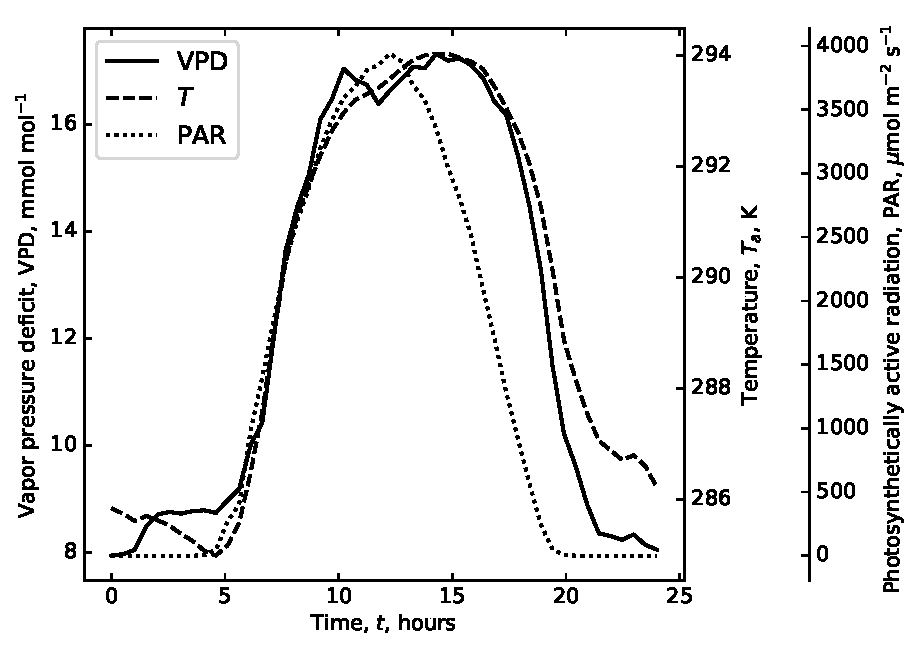
\includegraphics[scale=0.75]{environment.pdf}   
    \end{center}
    \caption{Diurnal trends of vapor pressure deficit (VPD), temperature ($T$), and photosynthetically active radiation (PAR). These are the averaged trends using measurements from the FLUXNET project at the Blodgett forest over 100 days starting from 5-29-2004 (the start of 4-months drought). These trends are repeated for the desired simulation duration.}
    \label{fig:environment}
\end{figure}

% \begin{figure}[h]
%     \begin{center}
%          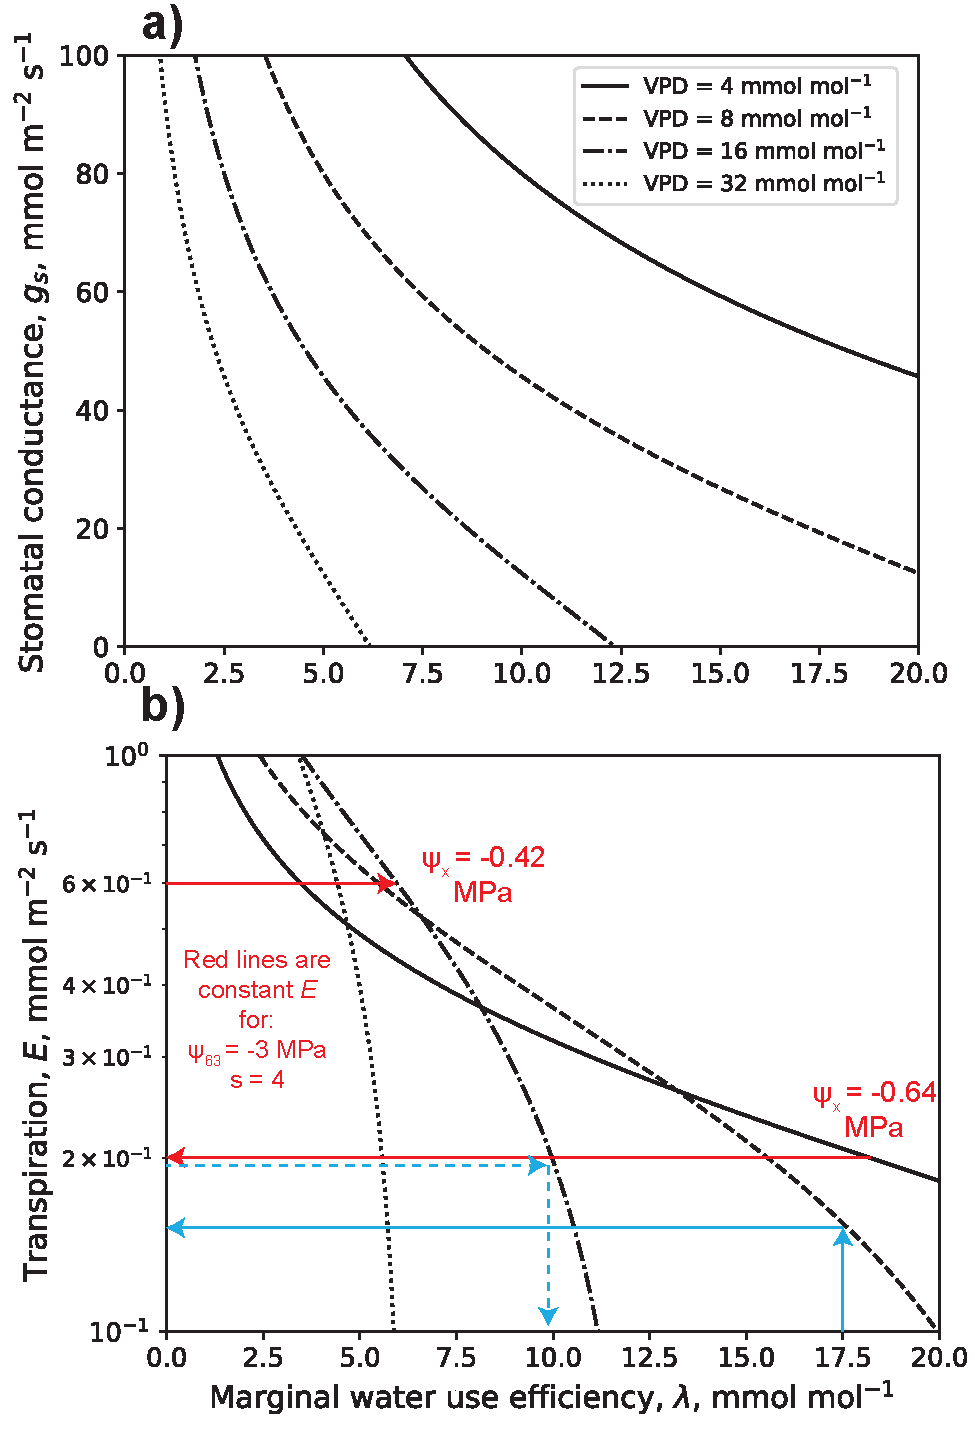
\includegraphics[scale=0.5]{g_E_lam_noon.pdf}   
%     \end{center}
%     \caption{a) Phase space of stomatal conductance $g_s$ vs the marginal water use efficiency $\lambda$ as a result of equation \ref{eqn:control} for different vapor pressure deficits (VPD). Other environmental conditions correspond to those shown in figure \ref{fig:environment} at noon and in table \ref{tab:props}. An increase in VPD or $\lambda$ both decrease $g_s$ with the other kept at constant. b) Transpiration $E$ corresponding to the curves in the phase space in panel a. An increase in $\lambda$ always leads to a decrease in $E$ when VPD is kept constant however the change in $E$ with changing VPD is more nuanced and depends on the value of $\lambda$. The solid blue arrows show how the value of $\lambda$ determines $E$ when transpiration is demand driven. When transpiration is supply limited, the maximum $E$ possible determines $\lambda$ as illustrated by the dashed blue arrows. Red horizontal arrows show the trends in $\lambda$ with changing VPD for supply limited transpiration of a plant with vulnerability curve (VC) parameters $\psi_{63}=-3$ MPa and $s=4$. The upper red arrow, showing constant $E$ at soil water potential $\psi_x = -0.42$ MPa, shows how $\lambda$ increases as the air dries from VPD$=4$ mmol mol$^{-1}$ to VPD$=16$ mmol mol$^{-1}$. The trend reverses as VPD continues increasing to $32$ mmol mol$^{-1}$. At $\psi_x = -0.64$ MPa, the trend in $\lambda$ reverses as shown by the lower red line. One can then trace these $\lambda$ trends to $g_s$ in panel a and infer magnitudes of midday stomatal closure and day to day $g_s$ sensitivity to drought.}
%     \label{fig:gs_E_lam}
% \end{figure}

\begin{figure}[h]
    \begin{center}
         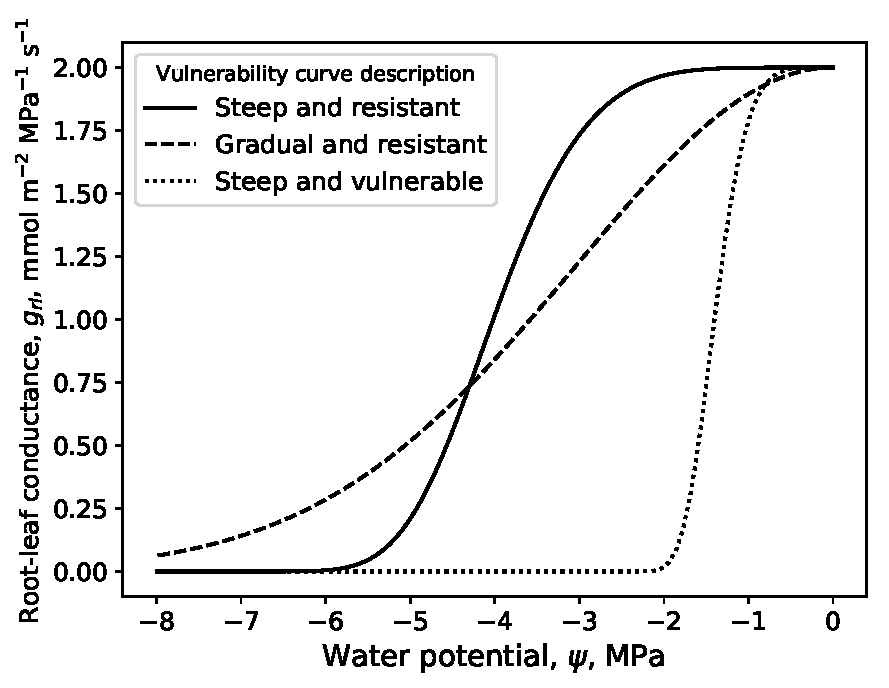
\includegraphics[scale=0.75]{grl.pdf}   
    \end{center}
    \caption{Loss of conductance curves for the three plants simulated throughout this work. The steep and resistant vulnerability curve has parameters $\psi_{63} = -4.3$ MPa, $s=5.4$, and $g_{rl,max} = 2$ mmol m$^{-2}$ MPa$^{-1}$ s$^{-1}$, the gradual and resistant has $\psi_{63} = -4.3$ MPa, $s=2$, and $g_{rl,max} = 2$ mmol m$^{-2}$ MPa$^{-1}$ s$^{-1}$, and the steep and vulnerable has $\psi_{63} = -1.5$ MPa, $s=5.4$, and $g_{rl,max} = 2$ mmol m$^{-2}$ MPa$^{-1}$ s$^{-1}$.}
    \label{fig:grl}
\end{figure}

\begin{figure}[h]
    \begin{center}
        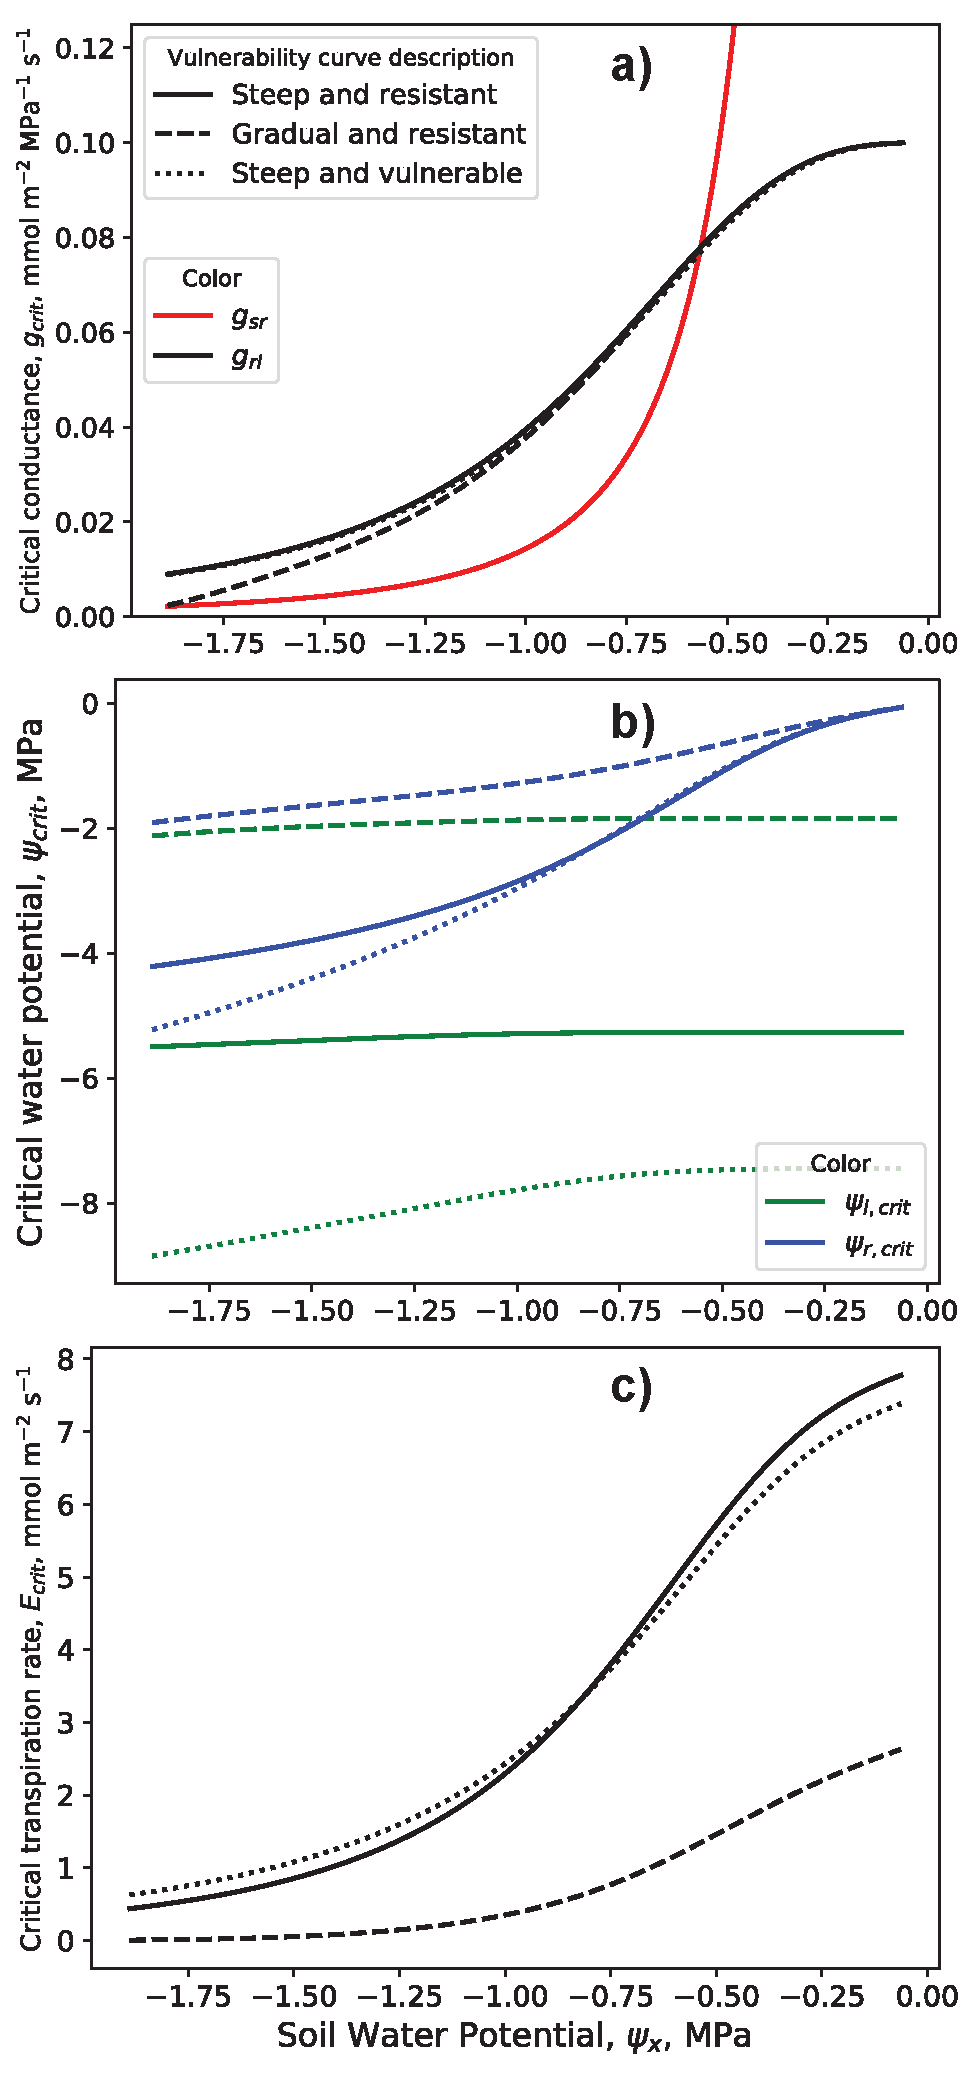
\includegraphics[scale=0.5]{g_psi_E_psix.pdf}
    \end{center}
    \caption{a) Soil to root conductance of the rhizosphere ($g_{sr}$) and root to leaf conductance of the plant ($g_{rl}$) that critical transpiration rate $E_{crit}$ for difference soil water potentials $\psi_x$. Soil is sandy loam and particular hydraulic parameters are shown in table \ref{tab:props}. Three vulnerability curve (VC) examples give different $g_{rl}$ trends. The VCs are described and plotted in figure \ref{fig:grl}. b) Critical root and leaf water potentials ($\psi_r$ and $\psi_l$, respectively) for the three VCs and for the particular soil type. The gradual and resistant VC ($s=2$) can maintain a gap between $\psi_r$ and $\psi_l$ as $\psi_x$ decreases unlike the other two VCs. c) The critical transpiration rates $E_{crit}$ for the three VCs. Details on how these curves were derived are available in the main text}
    \label{fig:gmax_Emax_psix}
\end{figure}

\begin{figure}[h]
    \begin{center}
         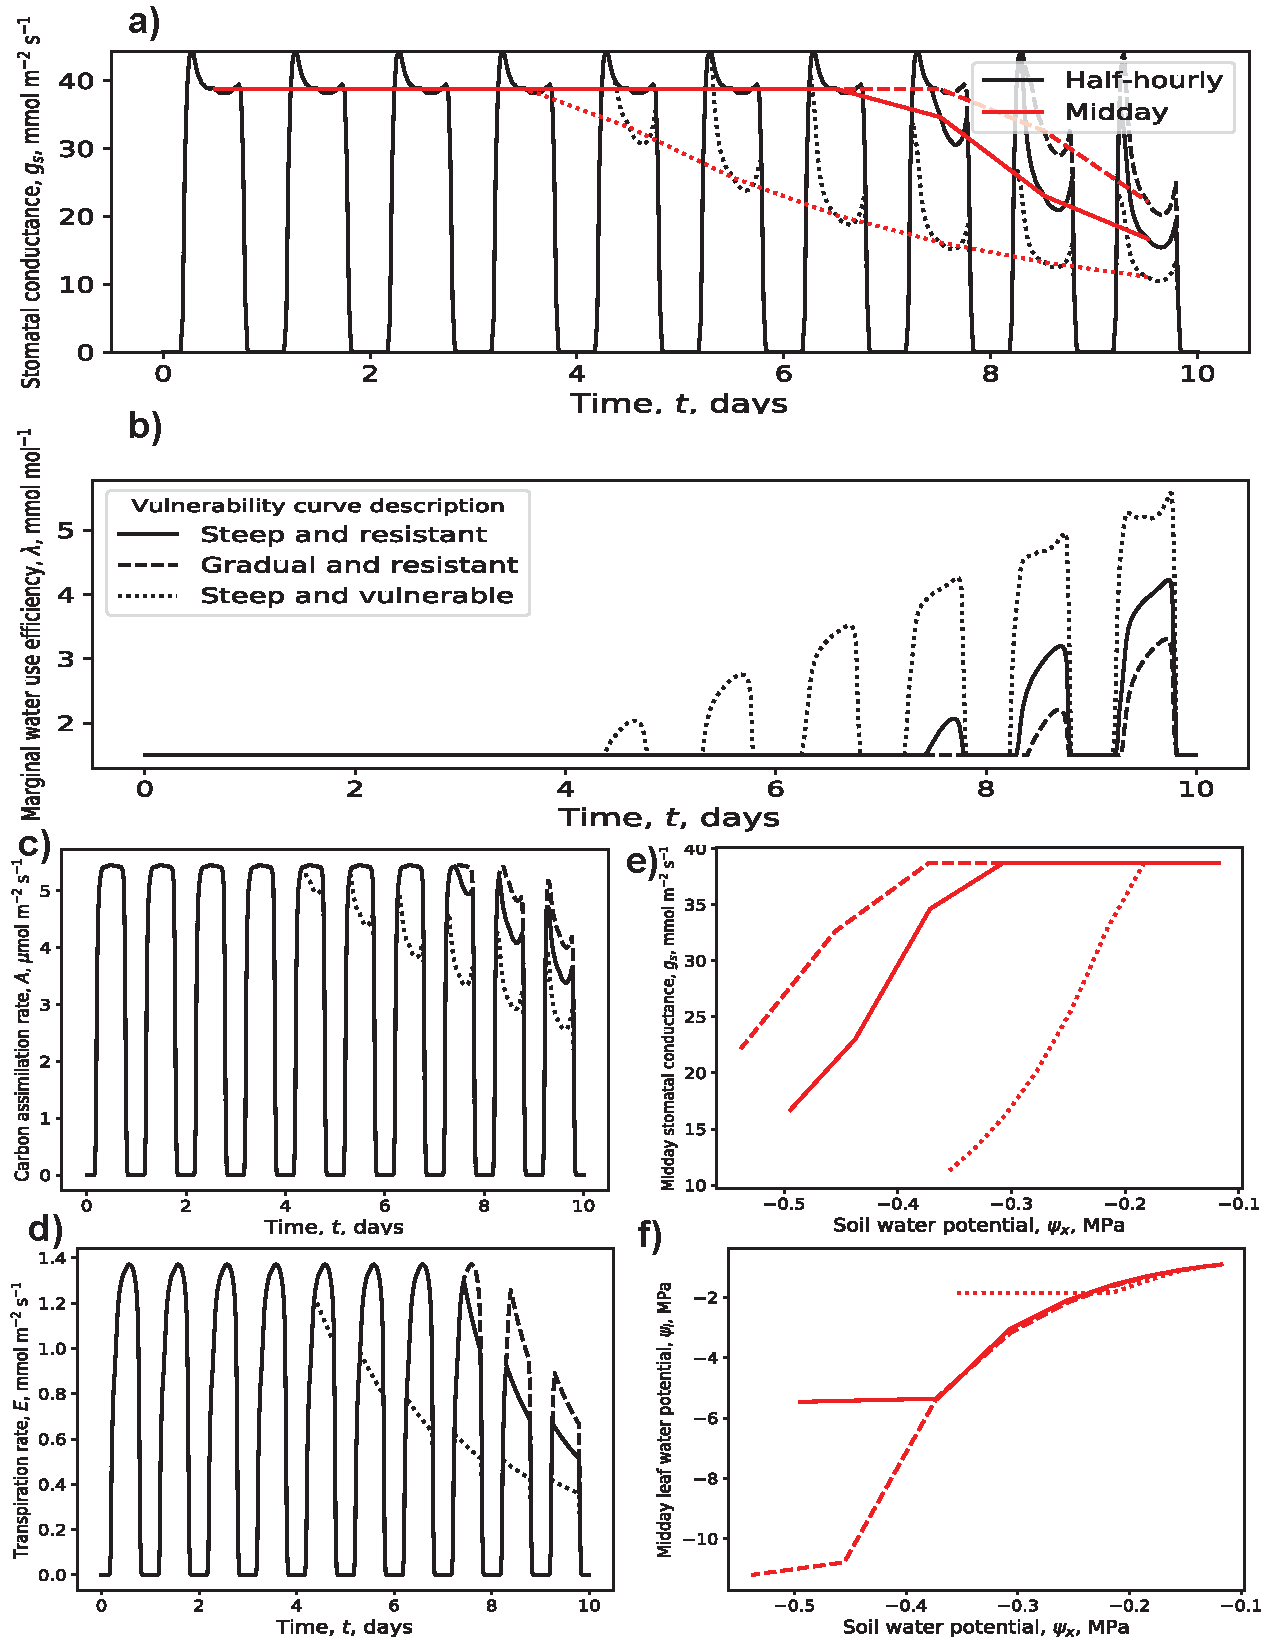
\includegraphics[scale=0.65]{WUS_no_comp.pdf} 
    \end{center}
    \caption{Results of a simulation where at time $t=0$, soil moisture $x(0) =0.25$. There are no competitive soil water users and the terminal marginal water use efficiency is set at $\lambda(10) = 1.6$ mmol mol$^{-1}$. a) Half-hourly (black) and midday (red) trends of stomatal conductance ($g_s$) with $t$ and b) $\lambda$ with $t$. Trends are shown for the three vulnerability curves (VCs) described and plotted in figure \ref{fig:grl}. Other plant and soil parameters are listed in the table \ref{tab:props}. c) Carbon assimilation rate ($A$) and d) transpiration rate ($E$) with $t$. e) Midday $g_s$ and f) Midday leaf water potential $\psi_l$ with soil water potential $\psi_x$.}
    \label{fig:WUS_no_comp}
\end{figure}

\begin{figure}[h]
    \begin{center}
         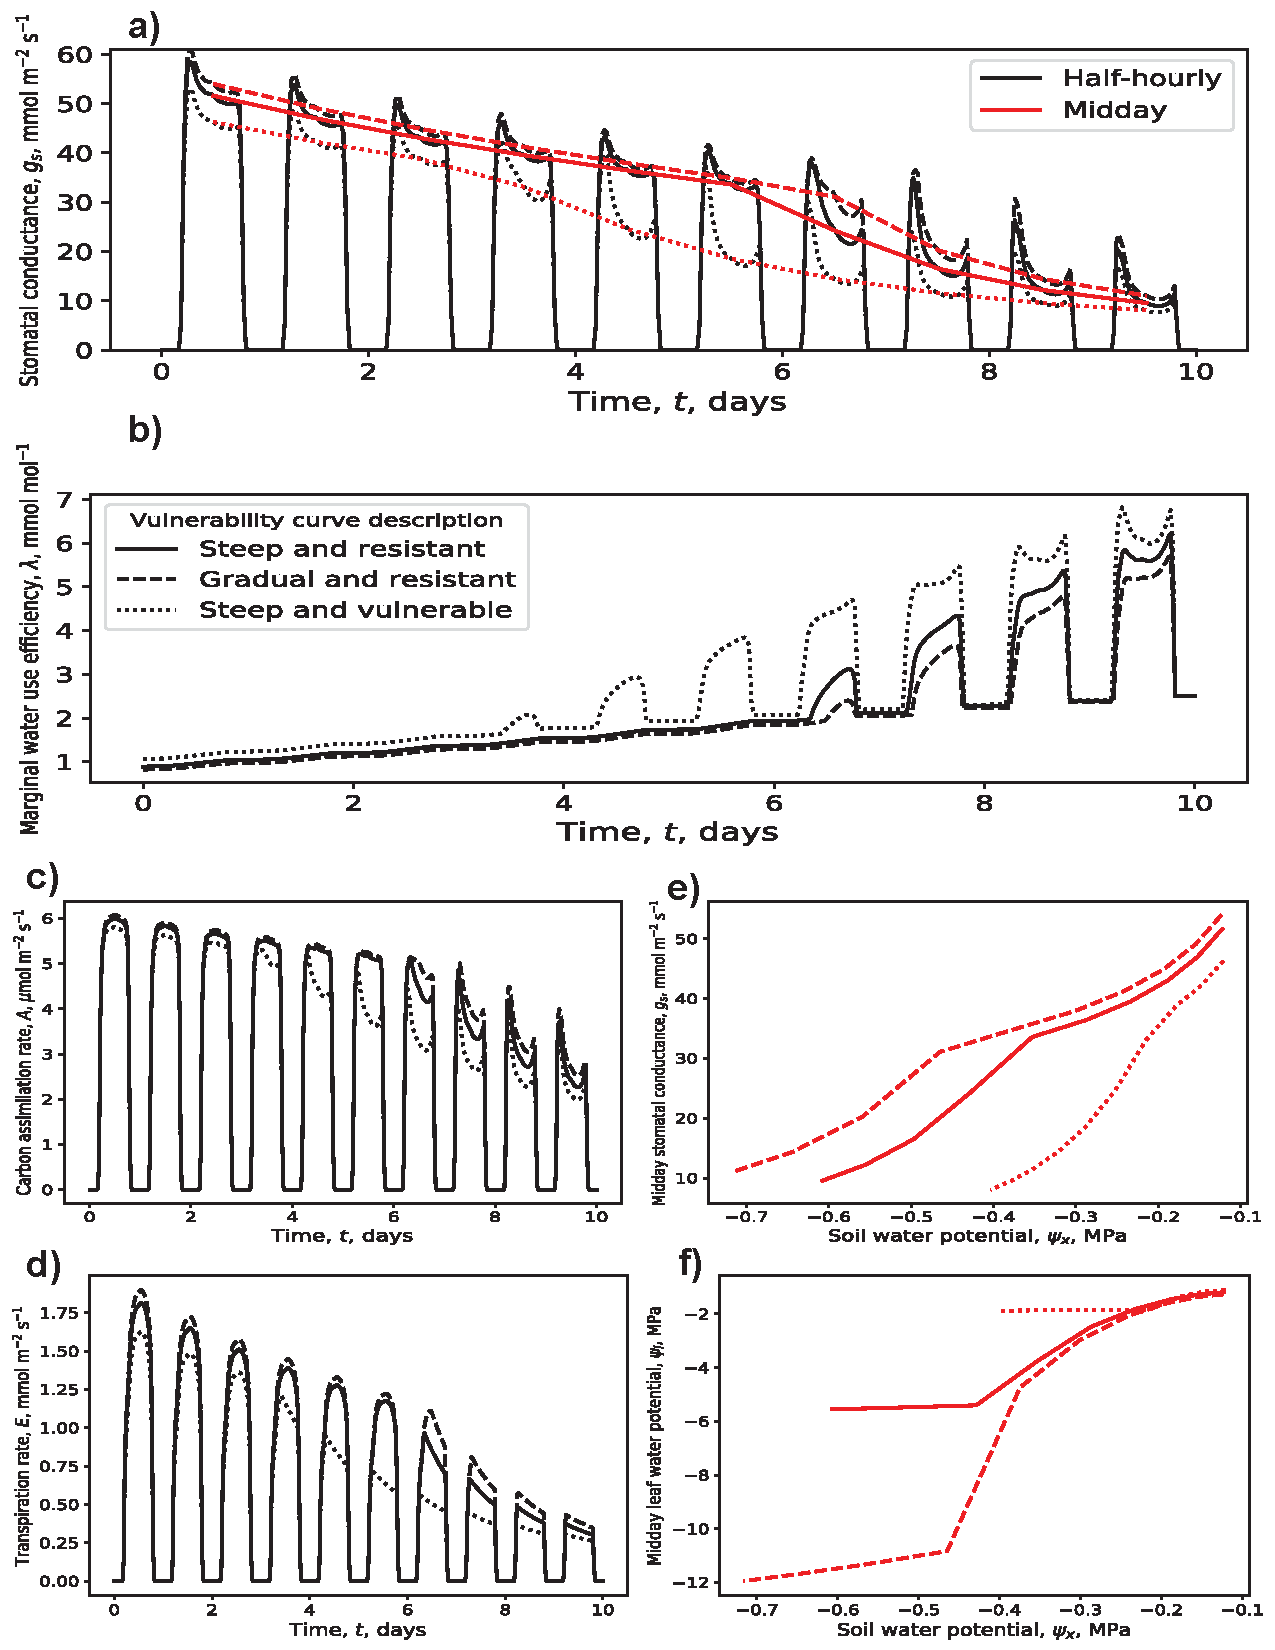
\includegraphics[scale=0.65]{WUS_comp.pdf}   
    \end{center}
    \caption{Results of a simulation where at time $t=0$, soil moisture $x(0) =0.25$. The terminal marginal water use efficiency is set at $\lambda(10) = 2.5$ mmol mol$^{-1}$. The competitive water sinks are soil free drainage and competing plants with similar vulnerability curves (VCs) and water use strategy (WUS) to those modeled. The competing plants have access to only 20\% of the root zone water of each modeled plant. a) Half-hourly (black) and midday (red) trends of stomatal conductance ($g_s$) with $t$ and b) $\lambda$ with $t$. Trends are shown for the three vulnerability curves (VCs) described and plotted in figure \ref{fig:grl}. Other plant and soil parameters are listed in the table \ref{tab:props}. c) Carbon assimilation rate ($A$) and d) transpiration rate ($E$) with $t$. e) Midday $g_s$ and f) Midday leaf water potential $\psi_l$ with soil water potential $\psi_x$.}
    \label{fig:WUS_comp}
\end{figure}

\begin{figure}[h]
    \begin{center}
         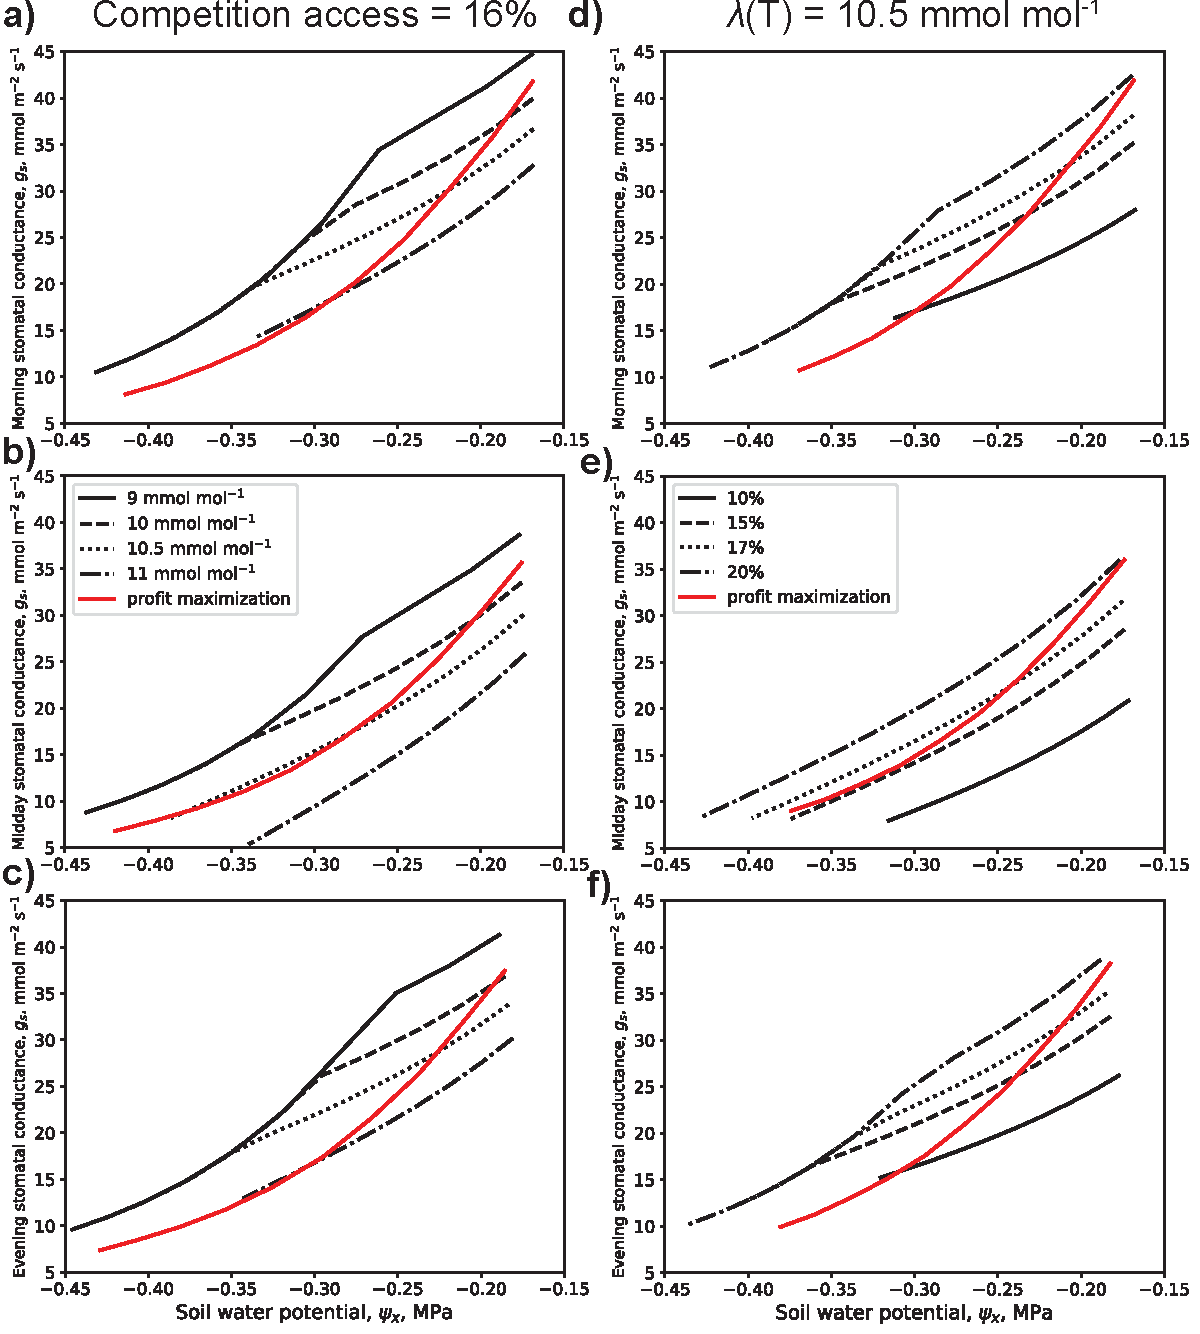
\includegraphics[scale=0.75]{profit_compare.pdf}   
    \end{center}
    \caption{Comparison between the dynamic optimality principle with plant hydraulic constraints and the profit maximization technique. In all panels, the vulnerable plant is modeled with vulnerability curve (VC) parameters $\psi_{63} = -1.5$ MPa, $s=4$, and $g_{rl,max} = 2$ mmol m$^{-2}$ MPa$^{-1}$ s$^{-1}$. The plant competes with plants of similar VC and behavior who have access to a certain percentage of the modeled plant's rooting zone water. This percentage is called the competition access percentage. Panels a,b, and c vary the terminal marginal water use efficiency $\lambda(T)$ at the end of drydown $t=T$ while keeping the competition access constant at 16\%. Panels a,b, and c like panels d,e, and f show the sensitivity of morning, midday, and evening  stomatal conductance $g_s$ to soil water potential $\psi_x$, respectively. Panels d,e, and f keep $\lambda(T) = 10.5$ mmol mol$^{-1}$ while varying the competition access.} 
    \label{fig:profit_compare}
\end{figure}


\clearpage

%%Figures, tables, and images will be published under a Creative Commons CC-BY licence and permission must be obtained for use of copyrighted material from other sources (including re-published/adapted/modified/partial figures and images from the internet). It is the responsibility of the authors to acquire the licenses, to follow any citation instructions requested by third-party rights holders, and cover any supplementary charges.

\subsection{Tables}
% Tables should be inserted at the end of the manuscript. Please build your table directly in LaTeX.Tables provided as jpeg/tiff files will not be accepted. Please note that very large tables (covering several pages) cannot be included in the final PDF for reasons of space. These tables will be published as \href{http://home.frontiersin.org/about/author-guidelines#SupplementaryMaterial}{Supplementary Material} on the online article page at the time of acceptance. The author will be notified during the typesetting of the final article if this is the case. 


\begin{table}[h]
    \centering
    \begin{tabular}{l l l l}
        Symbol & Description & Value & Unit \\
        \hline
        \multicolumn{4}{l}{}\\
        \multicolumn{4}{l}{\textit{Soil and root hydraulic properties}}\\
        \hline
        % \multicolumn{4}{l}{}\\
        $\psi_{sat}$ & Saturation water potential & -1.5 & kPa\\
        $\psi_x$ & Soil water potential & & MPa\\
        $x$ & relative soil moisture & & m$^{3}$ m$^{-3}$\\
        $g_{sr,max}$ & Maximum ground area specific soil-root conductance & $0.72 * 10^{-3}$ & kg s m$^{-3}$ \\
        $g_{sr}$ & Ground area specific soil-root conductance & & kg s m$^{-3}$\\
        $b$ & Power law dependence parameter with $\psi_x$ & 3.1 & \\
        $RAI$ & Root area index & 10 & m$^{2}$ m$^{-2}$\\
        $D_r$ & Average fine root diameter & 1 & mm \\
        $Z_r$ & Effective rooting depth & 0.3 & m\\ 
        $U$ & Uncontrolled losses of soil water & & mmol m$^{-2}$ s$^{-1}$\\
        \hline
        \multicolumn{4}{l}{}\\
        \multicolumn{4}{l}{\textit{Above-ground plant hydraulic properties}}\\
        \hline
        $g_{rl,max}$ & Maximum leaf area specific root-leaf conductance & 2 & mmol m$^{-2}$ s$^{-1}$ MPa$^{-1}$ \\
        $g_{rl}$ & Leaf area specific root-leaf conductance & see figure \ref{fig:grl} & mmol m$^{-2}$ s$^{-1}$ MPa$^{-1}$ \\
        $\psi_{63}$ & water potential at which $g_{rl} \approx 0.37 g_{rl,max}$ & see figure \ref{fig:grl} & MPa \\
        $s$ & Shape parameter of the vulnerability curve & see figure \ref{fig:grl} &  \\
        $g_s$ & Leaf area specific stomatal conductance & see figures \ref{fig:WUS_no_comp}, \ref{fig:WUS_comp} & mmol m$^{-2}$ s$^{-1}$ \\
        LAI & Leaf area index & 1.5 & m$^{2}$ m$^{-2}$\\
        \hline
        \multicolumn{4}{l}{}\\
        \multicolumn{4}{l}{\textit{Environmental properties}}\\
        \hline
        VPD & Vapor Pressure Deficit & see figure \ref{fig:environment} & mmol mol$^{-1}$\\
        $T_a$ & Atmospheric temperature & see figure \ref{fig:environment} & K \\
        PAR & Incoming photosynthetically active radiation & see figure \ref{fig:environment} & $\mu$mol m$^{-2}$ s$^{-1}$ \\
        \hline
        \multicolumn{4}{l}{}\\
        \multicolumn{4}{l}{\textit{Optimization results}}\\
        \hline
        $E(t)$ & Leaf area specific transpiration rate & & mmol m$^{-2}$ s$^{-1}$\\
        $A(t)$ & Leaf area specific carbon assimilation rate & & mmol m$^{-2}$ s$^{-1}$\\
        $\lambda (t)$ & Lagrange multiplier of the soil water balance constraint & & mmol mol$^{-1}$\\
        $L(t)$ & Augmented lagrangian & & mmol m$^{-2}$ s$^{-1}$\\
        $J$ & Objective function to be maximized & & mmol m$^{-2}$\\
        $T$ & Drydown period & 10 & days\\
    \end{tabular}
    \caption{Symbols of soil, plant, and environmental properties along with their description, typical values, and units. Values for specific simulations will be mentioned in the simulation description and in the corresponding figure caption.}
    \label{tab:props}
\end{table}


% \section{Nomenclature}

% \subsection{Resource Identification Initiative}
% To take part in the Resource Identification Initiative, please use the corresponding catalog number and RRID in your current manuscript. For more information about the project and for steps on how to search for an RRID, please click \href{http://www.frontiersin.org/files/pdf/letter_to_author.pdf}{here}.

% \subsection{Life Science Identifiers}
% Life Science Identifiers (LSIDs) for ZOOBANK registered names or nomenclatural acts should be listed in the manuscript before the keywords. For more information on LSIDs please see \href{http://www.frontiersin.org/about/AuthorGuidelines#InclusionofZoologicalNomenclature}{Inclusion of Zoological Nomenclature} section of the guidelines.


% \section{Additional Requirements}

% For additional requirements for specific article types and further information please refer to \href{http://www.frontiersin.org/about/AuthorGuidelines#AdditionalRequirements}{Author Guidelines}.

\section*{Conflict of Interest Statement}
%All financial, commercial or other relationships that might be perceived by the academic community as representing a potential conflict of interest must be disclosed. If no such relationship exists, authors will be asked to confirm the following statement: 

The authors declare that the research was conducted in the absence of any commercial or financial relationships that could be construed as a potential conflict of interest.

\section*{Author Contributions}

The Author Contributions section is mandatory for all articles, including articles by sole authors. If an appropriate statement is not provided on submission, a standard one will be inserted during the production process. The Author Contributions statement must describe the contributions of individual authors referred to by their initials and, in doing so, all authors agree to be accountable for the content of the work. Please see  \href{http://home.frontiersin.org/about/author-guidelines#AuthorandContributors}{here} for full authorship criteria.

\section*{Funding}
G. Katul, A. Mrad, M. Nakad, and J.C. Domec acknowledge support from the U.S. National Science Foundation (NSF-EAR-1344703,NSF-AGS-1644382, and NSF-IOS-1754893).

\section*{Acknowledgments}
This work used eddy covariance data acquired and shared by the FLUXNET community, including these networks: AmeriFlux, AfriFlux, AsiaFlux, CarboAfrica, CarboEuropeIP, CarboItaly, CarboMont, ChinaFlux, Fluxnet-Canada, GreenGrass, ICOS, KoFlux, LBA, NECC, OzFlux-TERN, TCOS-Siberia, and USCCC. The ERA-Interim reanalysis data are provided by ECMWF and processed by LSCE. The FLUXNET eddy covariance data processing and harmonization was carried out by the European Fluxes Database Cluster, AmeriFlux Management Project, and Fluxdata project of FLUXNET, with the support of CDIAC and ICOS Ecosystem Thematic Center, and the OzFlux, ChinaFlux and AsiaFlux offices.


\section*{Appendix: Mathematical derivations}
% Please see the availability of data guidelines for more information, at https://www.frontiersin.org/about/author-guidelines#AvailabilityofData

\bibliographystyle{frontiersinSCNS_ENG_HUMS} % for Science, Engineering and Humanities and Social Sciences articles, for Humanities and Social Sciences articles please include page numbers in the in-text citations
%\bibliographystyle{frontiersinHLTH&FPHY} % for Health, Physics and Mathematics articles
\bibliography{references}

%%% Make sure to upload the bib file along with the tex file and PDF
%%% Please see the test.bib file for some examples of references

% \section*{Figure captions}

% %%% Please be aware that for original research articles we only permit a combined number of 15 figures and tables, one figure with multiple subfigures will count as only one figure.
% %%% Use this if adding the figures directly in the mansucript, if so, please remember to also upload the files when submitting your article
% %%% There is no need for adding the file termination, as long as you indicate where the file is saved. In the examples below the files (logo1.eps and logos.eps) are in the Frontiers LaTeX folder
% %%% If using *.tif files convert them to .jpg or .png
% %%%  NB logo1.eps is required in the path in order to correctly compile front page header %%%

% \begin{figure}[h!]
% \begin{center}
% 
\includegraphics[width=10cm]{logo1}% This is a *.eps file
% \end{center}
% \caption{ Enter the caption for your figure here.  Repeat as  necessary for each of your figures}\label{fig:1}
% \end{figure}


% \begin{figure}[h!]
% \begin{center}
% \includegraphics[width=15cm]{logos}
% \end{center}
% \caption{This is a figure with sub figures, \textbf{(A)} is one logo, \textbf{(B)} is a different logo.}\label{fig:2}
% \end{figure}

%%% If you are submitting a figure with subfigures please combine these into one image file with part labels integrated.
%%% If you don't add the figures in the LaTeX files, please upload them when submitting the article.
%%% Frontiers will add the figures at the end of the provisional pdf automatically
%%% The use of LaTeX coding to draw Diagrams/Figures/Structures should be avoided. They should be external callouts including graphics.

\end{document}
